\documentclass[conference]{IEEEtran}


\usepackage{amsmath}
\usepackage{graphicx}
\usepackage[ruled,vlined,linesnumbered]{algorithm2e}
\usepackage{boxedminipage}
\usepackage{caption}
\usepackage{epstopdf}
\usepackage{tablefootnote}

 \let\labelindent\relax
\usepackage{enumitem}

\sloppy

% the fixme command
\newcommand{\fixme}[1]
{
  \noindent
  \begin{boxedminipage}{\linewidth}
    \textsl{{\bf FIXME: #1}}
  \end{boxedminipage}
}



\begin{document}

\title{Autoscaling Web Applications in Heterogeneous Cloud Infrastructures}

\author{\IEEEauthorblockN{Hector Fernandez}
\IEEEauthorblockA{VU University Amsterdam\\
Email: hector.fernandez@vu.nl}
\and
\IEEEauthorblockN{Guillaume Pierre}
\IEEEauthorblockA{IRISA / Rennes 1 University\\
Email: guillaume.pierre@irisa.fr}
\and
\IEEEauthorblockN{Thilo Kielmann}
\IEEEauthorblockA{VU University Amsterdam\\
Email: thilo.kielmann@vu.nl}}

\maketitle

\begin{abstract}
Improving resource provisioning of heterogeneous cloud infrastructures is an important research challenge. The wide diversity of cloud-based applications and customers with different QoS requirements have recently exhibited the weaknesses of current provisioning systems. Today's cloud infra\-structures provide provisioning systems that dynamically adapt the computational power of applications by adding or releasing resources. Unfortunately, these scaling systems are fairly limited: \emph{(i)} They restrict themselves to a single type of resource; \emph{(ii)} they are unable to fulfill QoS requirements in face of spiky workload; and \emph{(iii)} they offer the same QoS level to all their customers, independent of customer preferences such as different levels of service availability and performance. In this paper, we present an autoscaling system that overcomes these limitations by exploiting heterogeneous types of resources, and by defining multiple levels of QoS requirements. The proposed system selects a resource scaling plan according to both workload and customer requirements. Our experiments conducted on both public and private infrastructures show significant reductions in QoS-level violations when faced with highly variable workloads.

\end{abstract}


\section{Introduction}

Talk about wikipedia outage, traffic spikes and amazon outages "Popular websites crippled by hours-long Amazon cloud service outage"

Talk about vertical and horizontal scaling
Measuring instance performance
Multi instance infrastrucutres

Even if we use two level threshold there are traffic oscillations which cannot be handled by the system due to minimal variations. These minimal oscillations can sometimes be higher than the own infrastructure cost and degradate the user experience. In this paper, we try to minimize these by using a heterogonouer resource provisioning system. the cost of the infrastructure

Contribution:
App metrics instead of other system which hare limited to VM-level metrics. (Pluggable autoscaling service)
Real application and traces
Cost considerations.
Decision making scaling up/down out/in.
Dynamic load balancing
Measuring instance performance without additional resources

SLO fulfillment in order to avoid the cost of slo penalties.
Type of machines
SLO penalty -- different type of customers

Explain what is a scaling plan
\label{sec:introduction}

\section{Background}
\label{sec:relatedWorks}

There is a wide literature on issues related to dynamic resource provisioning for cloud web applications. Different approaches present solutions based on queuing models~\cite{urgaonkar_agile_2008}, feedback loops techniques~\cite{gong_gray-box_2010}, mathematical models~\cite{muppala_regression-based_2012} or even approaches using neural networks techniques~\cite{islam_empirical_2012}. However, most of these models require a deep understanding in mathematics or machine learning techniques which are not easily interpreted by non specialists. Besides the traffic in web applications is shaped by a combination of different factors such as diurnal and seasonal cycles, sociological and psychological, that follows an irregular pattern. It makes extremely challenging the design and development of realistic and accurate dynamic provisioning mechanisms. 

These well-known drawbacks force to IaaS like Amazon EC2 and Windows Azure~\cite{azure}, or PaaS like RightScale~\cite{right-scale} and OpenShift~\cite{openshift},  to design simple threshold rule-based auto-scaling systems, instead of relying on approaches from academic research. Unfortunately, these scaling systems are naive, wasteful in terms of resource consumption and cost savings, and an easy target for flash crowds.

% Workloads follow irregular patterns including “flash crowds".

% It is slow to workload changes and not effective at handling complex load
%patterns experienced in practice. Besides, over peak load reactive dynamic provisioning typically does no more than overprovisioning over one computing resource, while %the provisioning over other resources including storage and networking is not explicitly addressed or optimized.

In the following, we present some of the most relevant and realistic academic approaches that proposed dynamic resource provisioning mechanisms for multi-tier applications. 

%As we mentioned, offline and online profiling are promising techniques when handling unpredictable and temporal burstly workloads in web applications.  

In ~\cite{urgaonkar_agile_2008, urgaonkar_cataclysm:_2008}, the authors designed and implemented a predictive and reactive provisioning mechanism. They used a queuing model  G/G/1 to decide the server pool size to be provisioned, and an admission control mechanism to face extreme workload variations. Offline prolifing techniques were employed to gather information about the resource requirements of the incoming requests for each tier, and thereby to selectively admit/reject requests for the lightweight files.  An evaluation using real-traces on a homogeneous infrastructures shows the benefits of this approach when handling flash crowds. Unfortunately, its admission control mechanism incurs into sporadic SLA violations ( if the server utilization exceed a pre-defined threshold) reducing the QoS of the service, and therefore affecting user experience. Similarly to the previous work, \cite{wang_appraise:_2009} extended queuing models and transaction mix models to design a predictive and reactive provisioning system. To model the application performance, they integrated proactive control and feedback control methods that dynamically adjusted the CPU capacity allocated to servers. This work only considered SLA constraints at the hardware level, while others constraints at the application level such as response time and request rate were not taken into consideration. Besides, an evaluation of CPU variations on a homogeneous infrastructure, when processing traces from a non real-world application, lack arguments to valid its approach.

%control and dynamic provisioning components in addition to the load balancing algorithm. It applies admission control to make sure flash crowd requests
%will not overload the provisioned server pool by dropping requests, and uses queuing-model based dynamic provisioning technology.

Regarding the management of flash crowds~\cite{zhang_resilient_2009}, a proactive application workload manager was designed to separate the user requests between two groups of servers:  one  named  'base workload'  referred to the smaller and smoother variations in the workload; and the other 'tresspassing' referred to the temporal burstly workloads caused by flash crowds. To do this, the authors attempt to divide the data items into popular and less popular, and place them in the right group of servers. Even tough a realistic evaluation was conducted on Amazon EC2 utilizing real traces (Yahoo video streaming), authors do not explain in details how the dynamic resource provisioning is done. Recently, in  \cite{kaviani_profiling-as--service:_2011}, online profiling techniques have been utilized for managing the tradeofff between performance overload, and cost savings for dynamic resource provisioning. The authors replicate at runtime a regular server hosting an application, with a new server with profiling instrumentation. Their experimental results show how profiling techniques can be included in a resource provisioning system, without causing important response time delays or throughput alterations in comparison with non-profiling provisioning. As we mentioned in Section~\ref{}, profiling techniques can report more benefits than  performance degradations or expenses.




%\section{Problem statement}
%\label{sec:motivation}

%%  ENVIRONMENT,  PROBLEM -- SLO FULFILLMEMT %%
The two main steps in resource provisioning are the decision of when to allocate resources and the selection of appropriate resources.
Accordingly, the most important and challenging step is the selection of an appropriate scaling plan that satisfies the performance requirements with an acceptable operational cost. 
To overcome this step, scaling systems have to take into consideration: the customer preferences in terms of QoS requirements and the resource heterogeneity.

A first problem in autoscaling systems arises when having to choose the scaling plan that better enforces the QoS requirements. Customer requirements, such as availability and performance, directly affect to the definition of a scaling plan, and therefore have to be considered when selecting a hardware configuration.

%Cloud infrastructures allows tenants to rent resources in a \emph{pay-as-you-go} fashion. This pricing model is specifically employed by enterprise software systems where the assurance of QoS requirements is crucial to boost the volume of customers, and hence their revenues. Typically these requirements are specified by the enterprise (customer) and affirmed by cloud provider, and vary depending on the size of the enterprise. Thus, large enterprises such as (e.g. Amazon, Twitter and eBay), pay more to provide high assurance of availability and performance to their clients; while small enterprises pay less to obtain an acceptable performance but with little service availability. When dealing with web applications, the achievement of these requirements become more complex, as the workload demand fluctuates as a result of sudden changes in the popularity, workload mix or caused by flash crowds, outages and network misconfigurations. These traffic anomalies are specifically difficult to handle by traditional systems, thus causing long periods of unsatisfactory fulfillment of the requirements. Failure to comply with satisfying these requirements are often associated with significant financial penalties or other forms of loss of revenue such as decreased in the user base. Hence, a first problem in autoscaling systems arises when having to choose the scaling plan that better enforces the QoS requirements. 

% A problem in autoscaling systems arises when handling the mentioned traffic anomalies in order to enforce the requirements.

%%  PROBLEM -- SCALING PLAN, RESOURCE HETEROGENEITY %%
Consequently, and regarding the cloud infrastructures, another problem in autoscaling comes up when deciding the right hardware configuration that will enforce these requirements over time. Cloud infrastructures are highly heterogeneous offering a wide diversity of server configurations for rent, each with a different infrastructure cost. As illustrated in Table~\ref{EC2instances} and Table~\ref{DAS4instances}, the pricing of servers can be generally defined by a linear function, where the cost per-server increases linearly with the number of cores. According to this resource classification, autoscaling systems can dynamically allocate and de-allocated servers with different hardware configurations to adapt the computing capacity to the service demand. For instance, gradually increasing workload volume can be handled by choosing a new configuration that minimizes the infrastructure cost of servers. In contrast, a sudden oscillation in workload caused by a flash crowd or outage will require additional capacity to be brought online as quickly as possible. Even though the diversity of hardware configurations is common in cloud infrastructures, the majority of autoscaling systems focus on minimizing the infrastructure cost rather than selecting a right combination of resources~\cite{urgaonkar_agile_2008,dejavu2012,herbst_2013}. This manner to proceed may lead to periods of unsatisfactory performance, specifically for applications that need to provide high availability to their clients. Note that, the use of low cost hardware configurations (\emph{e.g. small}) may suffer performance degradations caused by the interference between activities of other VM's allocated to the same physical server. In summary, the selection of the resulting scaling plan has to find the tradeoff between the service demand and the capacity of this new configuration to fulfill the requirements.

Given such a scenario, the goal of our work is to develop a system that supports elasticity for applications by choosing the most suited scaling plan according to the customer preferences.

% Even though the diversity of hardware configurations is common in cloud infrastructures, the majority of autoscaling systems focus on the decision of when to provision rather than in the selection of suited resources.

%% PROBLEM -- VM PERFORMANCE PROFILING -- %%

%Another problem with existing provisioning systems is that resource heterogeneity is not considered when deciding the type of server to provision. This imply that unappropriate scaling  decisions can be triggered adding or removing wrong size of resources causing SLO violations or increasing the operational cost. As detailed in , the use of profiling techniques, while the application is in use, improve the accuracy of the decisions by creating performance profiles of the resources.













%\label{sec:motivation}

\section{Autoscaling system architecture}
\label{sec:proposed_approach}

The proposed autoscaling system scales a web application in response to change in throughput at fixed intervals, which we denote by reconfiguration intervals set to 10 minutes.  This system operates alongside the services deployed by ConPaaS, an open-source runtime environment for hosting applications in Cloud infrastructures~\cite{conpaasIC}. Nevertheless, it can also be easily integrated into any other PaaS, as it only relies on two common services provided by any platform: the resource manager and the monitoring engine. To feed this system, we use the monitoring engine that tracks the application-workload and system resources. Thus, as shown on Figure~\ref{autoScalingSys}, the architecture of our system has the following key components:

%aThis system is able to provision the right amount and type of resources for minimizing the number of SLA violations while keeping the operational cost adapted to the customer requirements.

%Vertical and horizontal scaling actions can be applicable to satisfy the service demand. 


%To choose a scaling plan, provisioning systems have to know the computing capacity of the different server configurations when running an application. To do that, the system creates profiles for each instance type by analyzing its performance behavior (e.g. measuring the cpu usage, request rate and response times). 

\textbf{Profiler:} This component was designed to measure the computing capacity of different hardware configurations when running an application. To do that, this component creates profiles for each resource type (VM instance in the following) by analyzing its performance behavior (e.g. the percentage of cpu usage, request rate and response time).  As we mentioned, the definition of profiles per-instance type improves the accuracy of the scaling actions, specifically in heterogeneous cloud infrastructures. Thus, the \emph{Profiler} component calculates the \emph{optimized throughput} of each type of provisioned configuration. Here an \emph{optimized throughput} is the performance pattern under which a resource assures the QoS requirements while avoiding its under/over-utilization.

% without any server instrumentation.




%However, this operation becomes more problematic by the fact that Web application workloads are often very unstable following an irregular pattern, with occasional short traffic spikes.

\textbf{Predictor:} To prevent SLA violations in advance, workload prediction is needed to estimate the incoming traffic. Inspired by~\cite{wolski_network_1999}, our \emph{Predictor} component takes the monitoring data as input and uses different time-series analysis techniques to predict the future service demand for the next monitoring window. To provide accurate forecasting measures, this component utilizes the technique that exhibited the lowest cumulative error measure during the previous monitoring window. By doing so, the \emph{Predictor} is able to adapt the predictions to the current type of workload. This component supports five distinct statistical models that fits four types of workload: \emph{(1)} \emph{Linear Regression} for linear trends~\cite{muppala_regression-based_2012}, \emph{(2)} \emph{Auto Regression Moving Average} (ARMA) for linear with small oscillations~\cite{roy_efficient_2011}, \emph{(3)} \emph{Exponential Smoothing Holt Winters} for daily and seasonal~\cite{exponential_smoothing2010}, and \emph{(4)} \emph{Autoregression} and \emph{Vector Autoregression} for correlated trends~\cite{chandra_dynamic_2003}. 




\textbf{Dynamic load balancer:} In order to adapt our system to the heterogeneity of requests and cloud resources, this component dynamically adjusts weights to the backend servers to proportionally distribute the incoming traffic based on the performance capacities of each provisioned resource. As an example, a server with four cores is able to process a higher number of requests, thus its weight is usually greater than a server with only one core.


\textbf{Scaler:} This component governs our autoscaling system. As illustrated in Figure~\ref{autoScalingSys}, the \emph{Scaler} uses the \emph{Predictor} and \emph{Profiler} components to find the scaling plan that fulfills a pre-established SLO, and consequently better enforces customer preferences. Furthermore, this component constantly analyzes the behavior of each provisioned VM, triggering the \emph{Dynamic load balancer} component when necessary.

\begin{figure}[t]
  \begin{center}
    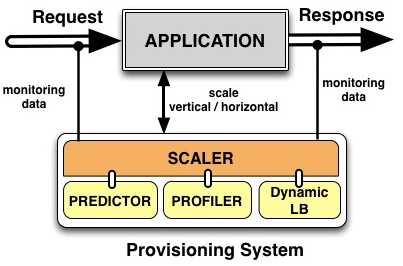
\includegraphics[width=.7\linewidth, height=3cm]{images/monitoringSchema}
  \end{center}
\vspace{-4mm}
  \caption{Autoscaling system.}
  \label{autoScalingSys}
\end{figure}

In the following section, we focus on answering \emph{when} to scale and \emph{which scaling plan} to choose when running web applications. Note that for simplicity, detailed description of the \emph{Predictor} and \emph{Dynamic LB} components are out of the scope of this work.

\section{Provisioning on demand}
\label{sec:decisionMaking}

The proposed autoscaling system scales a web application in response to change in throughput at fixed intervals, which we denote by reconfiguration intervals set to 10 minutes.  This system operates alongside the services deployed by ConPaaS, an open-source runtime environment for hosting applications in Cloud infrastructures~\cite{conpaasIC}. Nevertheless, it can also be easily integrated into any other PaaS, as it only relies on two common services provided by any platform: the resource manager and the monitoring engine. To feed this system, we use the monitoring engine that tracks the application-workload and system resources. Thus, the architecture of our system has the following key components:

%aThis system is able to provision the right amount and type of resources for minimizing the number of SLA violations while keeping the operational cost adapted to the customer requirements.

%Vertical and horizontal scaling actions can be applicable to satisfy the service demand. 


%To choose a scaling plan, provisioning systems have to know the computing capacity of the different server configurations when running an application. To do that, the system creates profiles for each instance type by analyzing its performance behavior (e.g. measuring the cpu usage, request rate and response times). 

\textbf{Profiler: } This component was designed to measure the computing capacity of the different server configurations when running an application. To do that, this component creates profiles for each server configuration (VM instance in the following) by analyzing its performance behavior (e.g. the percentage of cpu usage, request rate and response time).  The definition of profiles per-instance type improves the accuracy of the scaling actions, specifically in heterogeneous cloud infrastructures. Thus, the \emph{Profiler} component calculates the \emph{optimized throughput} of each type of provisioned configuration. Here an \emph{optimized throughput} is the performance pattern under which a resource assures the QoS requirements while avoiding its under/over-utilization.

% without any server instrumentation.




%However, this operation becomes more problematic by the fact that Web application workloads are often very unstable following an irregular pattern, with occasional short traffic spikes.

\textbf{Predictor: } To prevent SLA violations in advance, workload prediction is needed to estimate the incoming traffic. Inspired by~\cite{wolski_network_1999}, our Predictor component takes the monitoring data as input and uses different time-series analysis techniques to predict the future service demand for the next monitoring window. To provide accurate forecasting measures, this component utilizes the technique that exhibited the lowest cumulative error measure during the previous monitoring window. By doing so, the Predictor is able to adapt the predictions to the current type of workload. This component supports five distinct statistical models that fits four types of workload: \emph{(1)} \emph{Linear Regression} for linear trends~\cite{muppala_regression-based_2012}, \emph{(2)} \emph{Auto Regression Moving Average} (ARMA) for linear with small oscillations~\cite{roy_efficient_2011}, \emph{(3)} \emph{Exponential Smoothing} for daily and seasonal~\cite{exponential_smoothing2010}, and \emph{(4)} \emph{Autoregression} and \emph{Vector Autoregression} for correlated trends~\cite{vector_autoregression_2006,chandra_dynamic_2003}. 




\textbf{Dynamic load balancer: } In order to adapt our system to the heterogeneity of requests and cloud resources, this component dynamically assigns weights to the backend servers to proportionally distribute the incoming traffic based on the performance characteristics of each backend. As an example, a server with four cores is able to process a higher number of requests, thus its weight is usually greater than a server with only one core.


\textbf{Scaler:} This component governs our autoscaling system. As illustrated in Figure~\ref{autoScalingSys}, Scaler uses the \emph{Predictor} and \emph{Profiler} components to find the provisioning strategy that fulfills a pre-established SLO (Service Level Objective), and consequently better enforces the customer preferences. Furthermore, this component constantly analyzes the behavior of each provisioned VM, triggering the \emph{Dynamic load balancer} component when necessary.

\begin{figure}[t]
  \begin{center}
    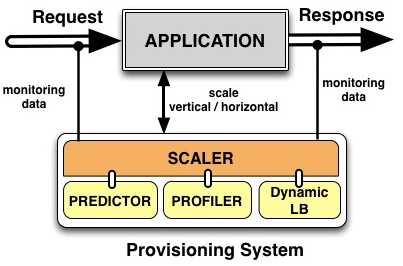
\includegraphics[width=.85\linewidth]{images/monitoringSchema}
  \end{center}
  \caption{Autoscaling system.}
  \label{autoScalingSys}
\end{figure}

In the rest of this section, we focus on answering when to scale and which scaling plan to choose when running web applications.

\subsection{Provisioning on demand}
As a central component of our autoscaling system, the Scaler component is responsible for triggering the scaling actions. It supports horizontal scaling as a technique to add and remove resources to an application. Horizontal scaling enables to create a cluster of virtual machines associated to one application, which size is dynamically adapted to the workload fluctuations by adding or removing resources to the cluster. Even though this scaling technique is commonly supported for the majority of resource provisioning systems~\cite{ali-eldin_2012,bunch_2012,urgaonkar_agile_2008}, our approach is able to use the resource heterogeneity of the cloud infrastructures to improve the efficiency of the scaling actions.

In order to decide when to trigger a scaling action, our system uses the following three methods: 

% On the other hand, in our system, vertical scaling enables to add or remove resources with high or less cpu and memory using \emph{service live migration}. Using this mechanism, the Scaler migrates the hosted service (web applications) from one virtual machine to another with a better hardware configuration. To reduce the degradations caused by this type of migration or by the booting time of the new machine, the Scaler checks the proper functioning of the new machine in order to release the older one.


\begin{itemize}

\item \emph{Response time analysis:} A precise analysis of the monitoring data is crucial to minimize performance degradations that are sometimes omitted by traditional analytical methods such as the median, average or moving average. To extract precise information from the monitoring data  (e.g. response times) describing the performance behavior of an application, we decided to extend a known smoothing technique called \emph{Weighted Moving Average} (WMA). Using our extension for WMA, it analyzes the monitoring data associating weights in an increasing order giving more importance to the latest monitoring data; and second it increments the original weight value of each data-point that exceeds the performance requirements. The weight increment can be modified to rise the awareness of the system to SLO violations  (in our experiments this increment was twice the original weight). By doing so, our system analyzes the monitoring data giving special importance to the data points on which SLO violations have occurred, and thereby is able to detect and avoid the maximum number of violations.

\item \emph{Definition of a reactive threshold:} Additionally to the fixed SLO threshold pre-defined by the QoS requirements (maximum response time), our system also includes an extra threshold (based on these requirements) that will enable in advance to react against any traffic variation, minimizing the number of SLO violations, or under-utilization of the provisioned resources. As illustrated in Figure~\ref{thr}, this reactive threshold specifies one upper and lower boundaries creating two head-rooms between them and the fixed threshold pre-defined by the user.

\begin{figure}[t]
  \begin{center}
    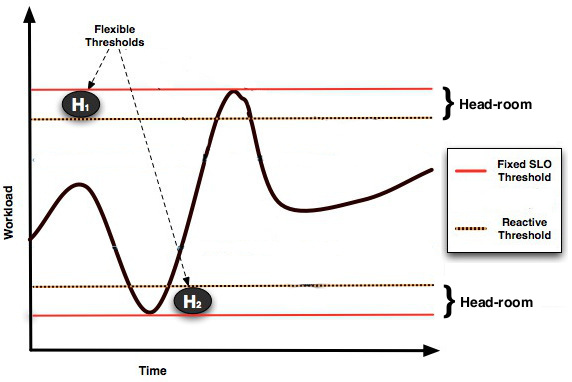
\includegraphics[width=.85\linewidth]{images/thresholdGraphic}
  \end{center}
  \caption{Reactive threshold.}
  \label{thr}
\end{figure}

\item \emph{Workload forecasting: }  The \emph{Predictor} component is utilized to trigger short-term forecasts operations that will minimize the number of future SLA violations, as well as keeping a high level of efficiency in the predictions. 
\end{itemize}

Based on these techniques, the \emph{Scaler} evaluates whether the current performance behavior requires triggering any of the following scaling actions:

\begin{itemize}

\item \textbf{Scale out:} Additional resources are provisioned if the loaded system state (response time or cpu utilization) exceeds the upper threshold, and the \emph{Predictor} confirms that such traffic changes will remain at least during the next monitoring window. In our experiments, we define monitoring windows of 5 minutes due to this interval is the minimum necessary time to collect fresh data from the monitoring engine provided by ConPaaS. 

\item \textbf{Scale back:} Resources are released if the loaded system state exceeds the lower threshold, and the \emph{Predictor} confirms that such traffic changes will remain at least during the next monitoring window.

\end{itemize}



%\subsubsection{Response time analysis - Time-series smoothing}

%When minimizing the SLA violations, a precise analysis of the monitoring data is crucial to improve the accuracy of the scaling decisions. It allows to %identify the resource requirements from the current workload type. This analyisis has even more importance when hosting web applications (e.g. %Wikipedia, Amazon) that need to provide high availability and performance to their clients. Moreover, the workload heterogeneity of this sites requires a %meticulous analysis of every monitoring data-point to reduce at the maximum the number of SLO violations. 

%\begin{figure}[htb]
%	\begin{minipage}[b]{0.49\linewidth}
%		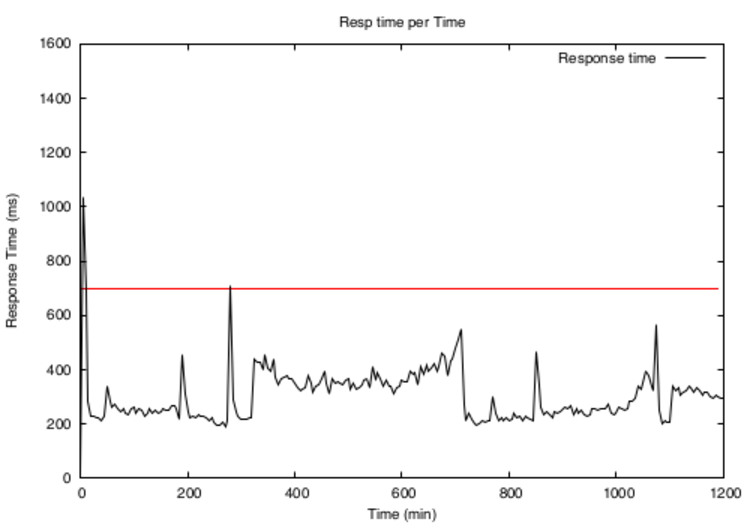
\includegraphics[width=4cm,height=3cm]{images/data2007/proxy_outputAvg.pdf}	
%		\vspace{-4mm}
%	\end{minipage}
%	\hfill
%	\begin{minipage}[b]{0.49\linewidth}
%		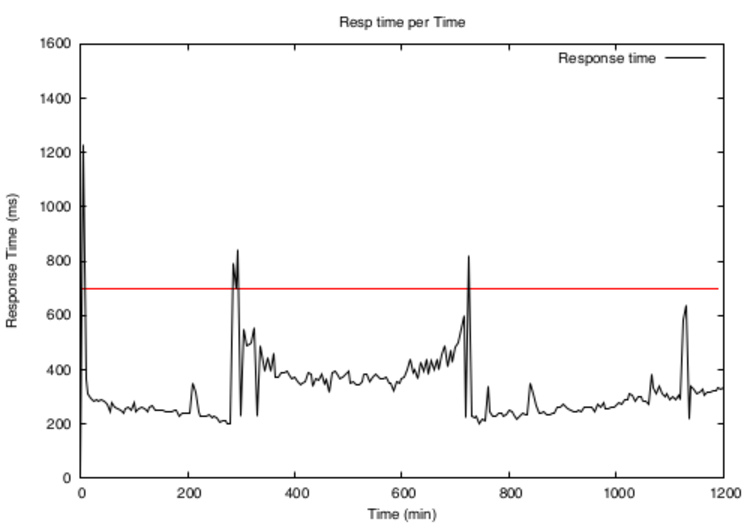
\includegraphics[width=4cm,height=3cm]{images/data2007/proxy_outputWMA.pdf}
%		\vspace{-4mm}
%	\end{minipage}
%\caption{Response times for a trace: Average vs extended WMA.}
%\label{fig:data_analysis}
%\end{figure}

%To obtain precise information (response times) that reflects the performance behavior of an application, we decided to extend a known smoothing technique called \emph{Weighted Moving Average} (WMA). This technique is widely used in resource provisioning systems instead of others such as the median, average or moving average. Using our extension of WMA, it first associated weights in an increasing order giving more importance to the latest monitoring data; and second it doubles the original weight value of each data-point that exceeds the performance requirements (response time). By doing so, the Scaler analyzes the monitoring data giving special importance to the data points on which SLO violations have occurred, and thereby being able to detect and avoid the maximum number of violations. As an example, Figure~\ref{fig:data_analysis} shows how several SLO violantions are omitted when analyzing the monitoring data using an average analytical method (left) than when using our version of WMA (right).

%\subsubsection{Definition of a reactive threshold}

%\fixme{Perhaps, you may want to omit this subsection, as it is more related to When to provision than How to provision ?}

%Initially, the user defines several performance requirements that will be utilized by the Scaler to trigger scaling actions. As we mentioned, these QoS goals are previously specified in the Service Level Objective (SLO). In particual, when hosting web applications, these performance requirements are usually related to the maximum processing time needed to serve any request (response times). Regarding SLO fulfillment the majority of resource provisioning system aims to maintain the processing time as closer as possible to the performance requirements. However, this operation can become a problem, as provisioning systems are vulnerable to temporal traffic oscillations causing SLO violations.

%Therefore, and based on the requirements, the Scaler defines a reactive threshold that will enable in advance to react against any traffic oscillation minimizing the number of SLO violations or period of time under-utilization of the provisioned resources. As shown in Figure~\ref{threshold}, this reactive threshold specifies one upper and lower boundaries creating two head-rooms between them and the performance requirements pre-defined by the user (for the response time). In the future, these two boundaries could be adjusted depending on the hardware configuration of each provisioned vm, as introduced in~\cite{beloglazov_adaptive_2010}.  


%\begin{figure}[htb]
 % \begin{center}
  %  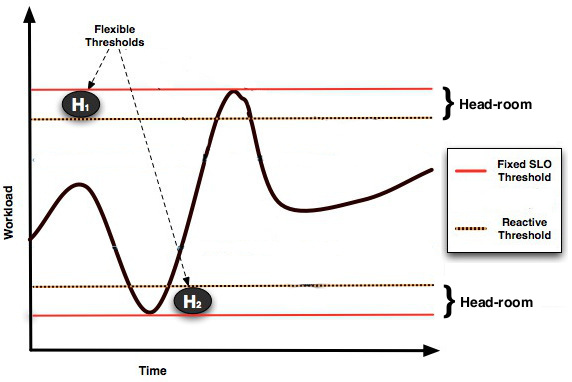
\includegraphics[width=.85\linewidth]{images/thresholdGraphic.jpg}
 % \end{center}
%\vspace{-5mm}
%  \caption{Reactive threshold.}
%  \label{threshold}
%\end{figure}



%\subsection{Online profiling of allocated instances\label{profiling}}
%\subsection{Measuring VM instance performance via online profiling\label{profiling}}

\subsection{Measuring VM instance performance \label{profiling}}

Regarding the resource heterogeneity of cloud infrastructures, a sensitivity analysis of the allocated resources is crucial to provide accurate scaling decisions. Accordingly, online profiling-based techniques~\cite{kaviani_profiling-as--service:_2011} have recently emerged as a solution to  estimate the resource's throughput under a certain workload. Traditionally, this technique replicates at runtime, a server hosting an application, with a new server with profiling instrumentation. To obtain  the profiling data, this new server analyzes the performance behavior of a specific resource under a fixed percentage of the incoming traffic~\cite{jiangThesis,dejavu2012}. The use of fixed workloads to calculate the maximum throughput of a resource do not necessary imply the definition of more accurate profiles. A reason seems to be the lack of ideal performance isolation in cloud infrastructures which affects the precision of the definitions, and consequently reduces the accuracy of the decisions. Furthermore, setting a profiling environment, in a heterogeneous cloud infrastructure, requires as many additional resources as number of available configurations. 

Even though the use of online-profiling techniques is still under study, the configuration of a parallel environment and the heterogeneity of the cloud resources are the major drawbacks for its adoption. These techniques increase the operational cost and do not necessarily improve the accuracy of the scaling decisions.

%Even though the use of online-profiling techniques is still under study, the configuration of a parallel %environment and the limited accuracy of its scaling decisions are the major drawbacks for its %adoption.

As a consequence, we designed a novel online profiling technique that gives an estimation of the optimized throughput of each allocated VM instance type without the need for additional resources or parallel environments. To do that, the \emph{Profiler} component use the provisioned resources for the analysis and estimation of the computing capacity of each available hardware configuration.

%Cpu.usage is relative to nominal frequency of the CPU’s – not the amount of time the CPU was busy, which is generally more relevant.

\begin{algorithm}
{\scriptsize
\SetAlgoLined
\SetInd{0mm}{2mm}
\KwData{ \\Service Level Objective, \emph{slo} \\ List of allocated VM instance types, \emph{inst\_types} \\ Compute units per \emph{inst\_type}, \emph{compute\_units$_{inst}$}}

\KwResult{VM instances performance classification, \emph{list\_perf}}

\While{ allocated instances to profile}{
\BlankLine
Collect profiling data of \emph{inst\_type}: \emph{req\_rate, \%cpu\_usage and resp\_time}\;

\While{ profiling data to smooth}{  \label{alg:smooth}
// Perform smoothing percentiles technique \;
\If{ \emph{resp\_time}$_i$ $>$ (slo * 0.25) and \emph{resp\_time}$_i$ $<=$ (slo * 0.75)}{ 
	\If{ \emph{req\_rate}$_i$ $>$ 0 and \emph{\%cpu\_usage}$_i$ $<$ 75}{ 
		\hspace{3mm} Add \emph{\%cpu\_usage$_i$} to \%cpu\_usage\_data\;
		\hspace{3mm} Add \emph{req\_rate$_i$} to req\_rate\_data\;
		\hspace{3mm} Add \emph{resp\_time$_i$} to resp\_time\_data\;
}
}
} \label{alg:endSmooth}
\BlankLine
Initialize instance capacity \emph{Ideal\_Throughput$_{inst}$} to 0 \;
\uIf{ \emph{resp\_time\_data}, \emph{\%cpu\_usage\_data}, \emph{req\_rate\_data}  \textbf{not empty}}{
Calculate average of \emph{\%cpu\_usage\_data}, \emph{\%CPU\_usage$_{inst}$} \; \label{alg:throughput_start}
Calculate average of \emph{req\_rate\_data}, \emph{Num\_requests$_{inst}$} \;
\BlankLine
\emph{Ideal\_Throughput$_{inst}$} = $\dfrac{ \bigg( \dfrac{\emph{\%CPU\_usage$_{inst}$} } {100} \bigg)} {\emph{Num\_requests$_{inst}$ } }$  \; \label{alg:throughput_end}
\BlankLine
Store instance computing capacity, \emph{Ideal\_Throughput$_{inst}$} \; 
}
\Else{ 
	Use historic value of \emph{Ideal\_Throughput$_{inst}$} for \emph{inst\_type}\;
}
\BlankLine
// Classify \emph{inst\_type} based on its computing capacity \; \label{alg:clas}
\If{ Ideal\_Throughput$_{inst}$ == 0 }{
Use \emph{compute\_units$_{inst}$} of \emph{inst\_type} to rank \emph{inst\_type} in \emph{list\_perf}\;
}
\Else{ 
Use new value of \emph{Ideal\_Throughput$_{inst}$} to rank \emph{inst\_type} in \emph{list\_perf}\; \label{alg:end_clas}
}
}
}
\caption{VM instance profiling algorithm}
\label{profilingAlg}
\end{algorithm}

As detailed in Algorithm~\ref{profilingAlg}, once the \emph{Scaler} component decides to trigger a scaling action, the \emph{Profiler} component estimates the throughput of the allocated instances according to the following steps:

\begin{enumerate}
\item Collect the latest hour of monitoring data from each VM instance type. This data contains information about monitoring metrics such as the request rate, total percentage of cpu usage and response time, which provide enough feedback for the definition of instance profiles. In fact, when provisioning web applications, these metrics are commonly used to decide whether to trigger scaling actions or not \cite{smartscale_2012,urgaonkar_agile_2008}. Nevertheless, the network bandwidth and memory usage can also be collected to define instance profiles.


\item Perform a smoothing technique over the profiling data of each instance to remove the noise generated by traffic spikes. As pointed out in~\cite{gandhi_hybrid_2012}, when hosting web applications sudden changes in the workload, interference due to virtualization or OS activities may affect the precision of the profiling process. Hence, we decided to smooth the profiling data during the latest hour (or older if there is not enough data) to identify the performance capacity of each allocated VM instance type. In particular, the \emph{Profiler} extracts the smoothed 75th and 25th percentiles from the response times below the SLO in correspondence with the \emph{reactive threshold}; and 75th percentile from the percentage of cpu usage data-points. (See Lines \ref{alg:smooth}-\ref{alg:endSmooth}). Note that, we only use the 75th percentile from the cpu usage due to lower values in the cpu usage do not imply a system free of SLA violations. As an example, \emph{m1.small} instances can throw violations even under percentages of cpu usage lower than 25\%. This technique allows to identify the optimized throughput of each instance while enforcing the performance requirements and avoiding CPU saturation. 

As an example in Figure~\ref{fig:vm_performance1} and Figure~\ref{fig:vm_performance2}, we show the profiling data and percentiles for one "m1.small" and one "c1.medium" EC2 instance types during one hour. The gray areas represent the ranges of response times and cpu usage comprised by the percentiles. Red circles contain all data points that will be used to calculate the optimized throughput of one VM instance. As we mentioned above, some data points are excluded as they identify periods of time on which resources suffered from under-utilization or over-utilization (denoted by white areas). Furthermore, as shown in Figure~\ref{fig:vm_performance1}, a short number of data points are comprised between the percentiles for the "m1.small" instance. Its poor hardware configuration makes this instance type more vulnerable to sudden changes in the workload.

%and three red circles highlight several data-points on which the performance of the instance was optimal while enforcing the %SLO.

%\begin{figure*}[htb]
%	\begin{minipage}[b]{0.5\linewidth}
%		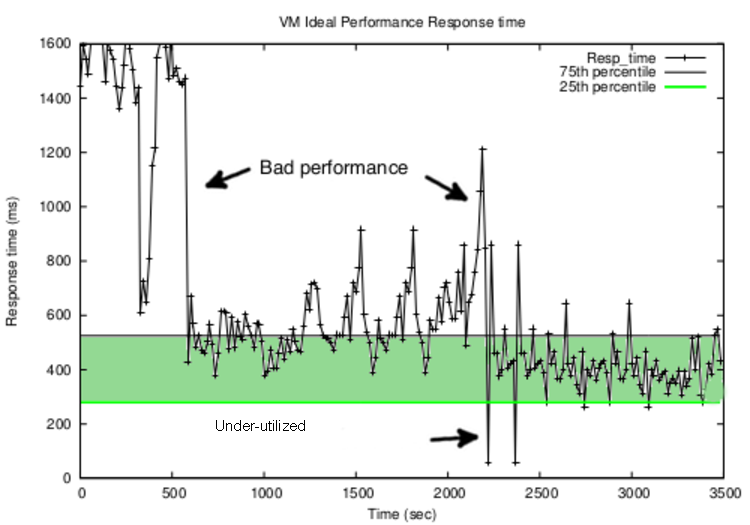
\includegraphics[height=4.5cm]{images/vm_performance_resp_smallEC2Remark.pdf}		%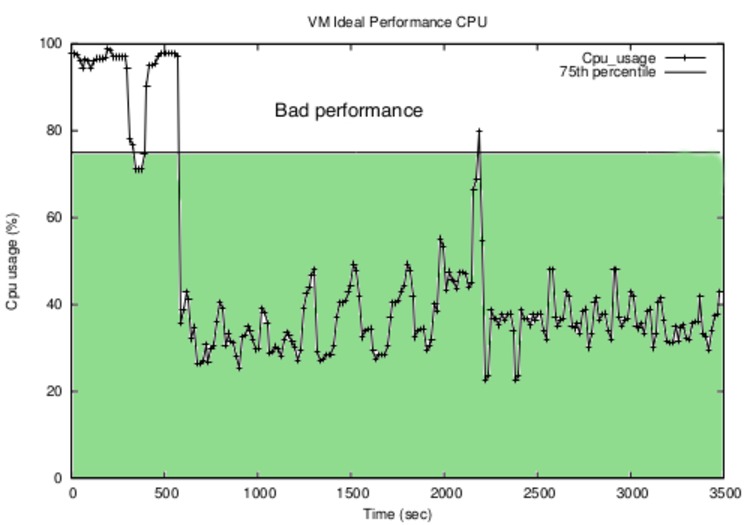
\includegraphics[height=4.5cm]{images/vm_performance_cpu_smallEC2Remark.pdf}
%		\vspace{-4mm}
%	\end{minipage}
%	\hfill
%	\begin{minipage}[b]{0.5\linewidth}
%		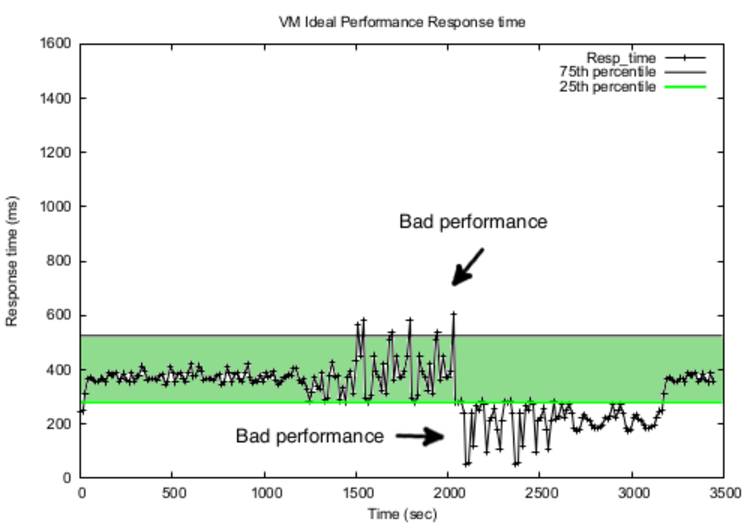
\includegraphics[height=4.5cm]{images/vm_performance_resp_c1mediumRemark.pdf}		%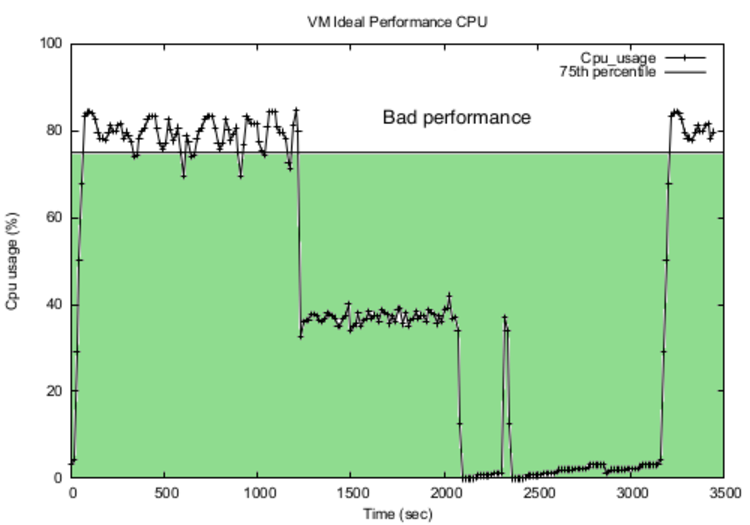
\includegraphics[height=4.5cm]{images/vm_performance_cpu_c1mediumRemark.pdf}
%		\vspace{-4mm}
%	\end{minipage}
%\caption{Profiling data and percentiles of m1.small and c1.medium EC2 instances.}
%\label{fig:vm_performance}
%\end{figure*}

\begin{figure}[t]
  \begin{center}
    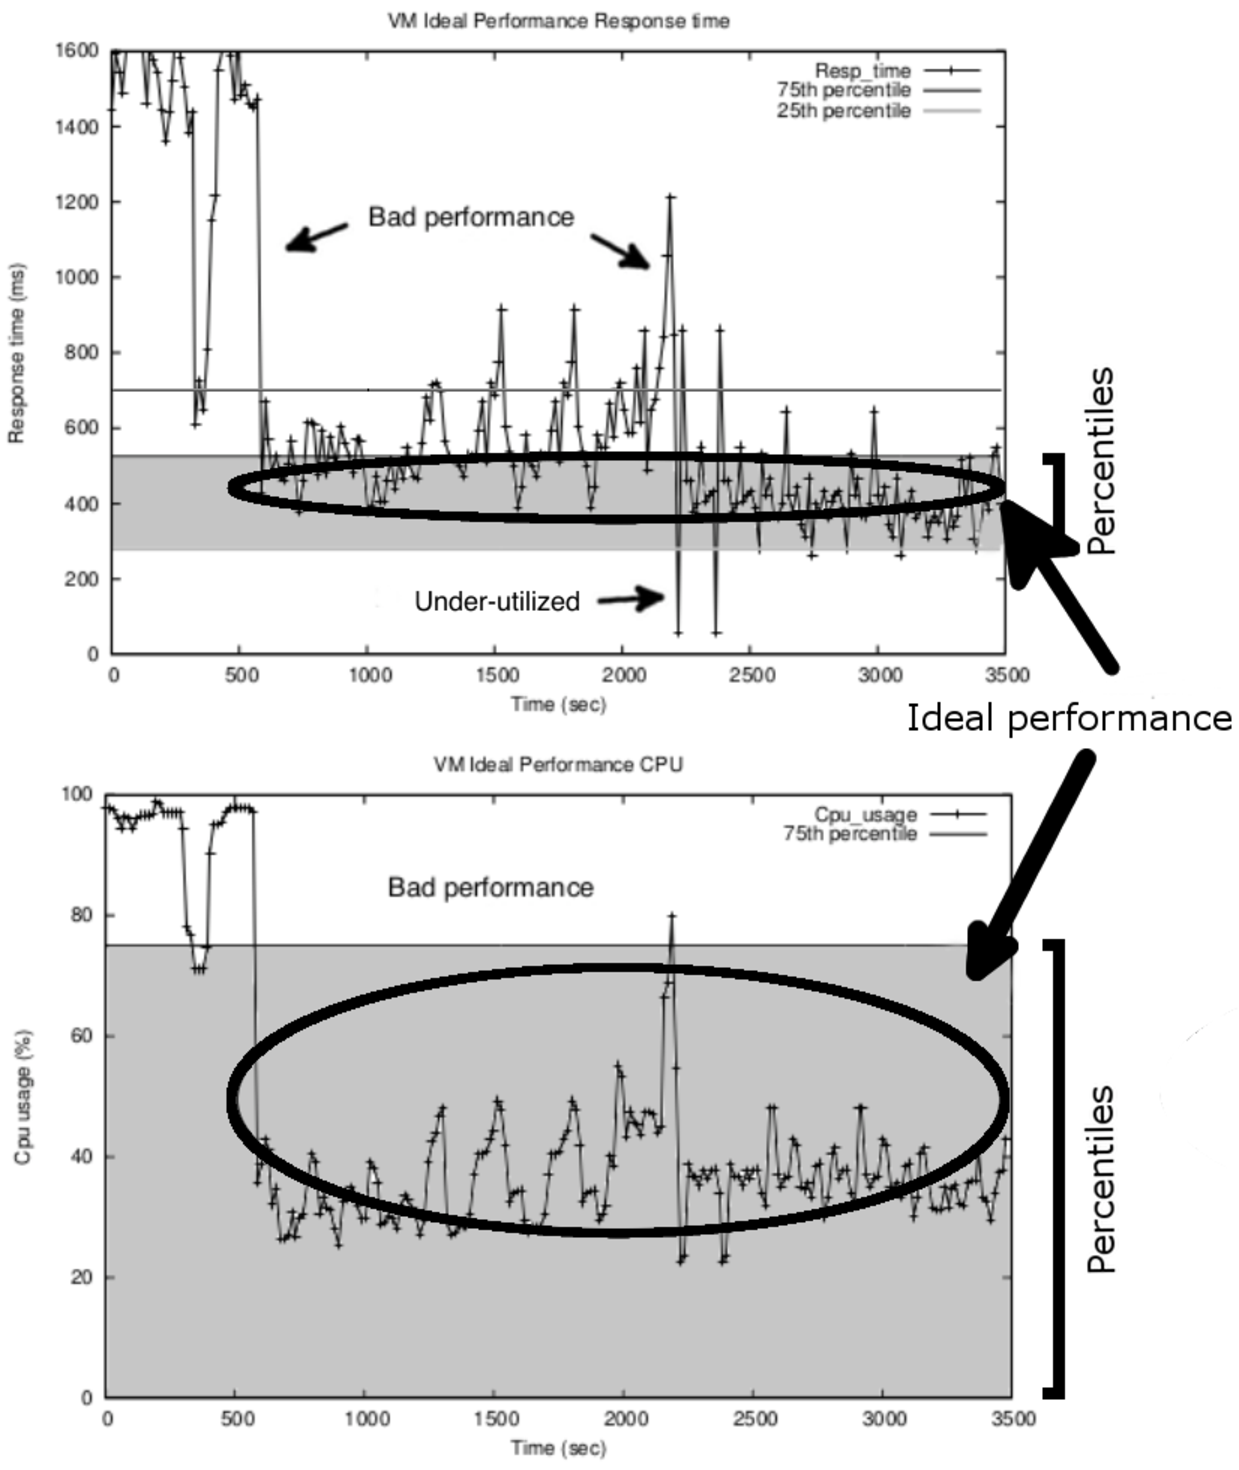
\includegraphics[width=\linewidth]{images/idealSmallRemark.pdf}
  \end{center}
  \caption{Profiling data and percentiles of m1.small.}
  \label{fig:vm_performance1}
\end{figure}

\begin{figure}[t]
  \begin{center}
    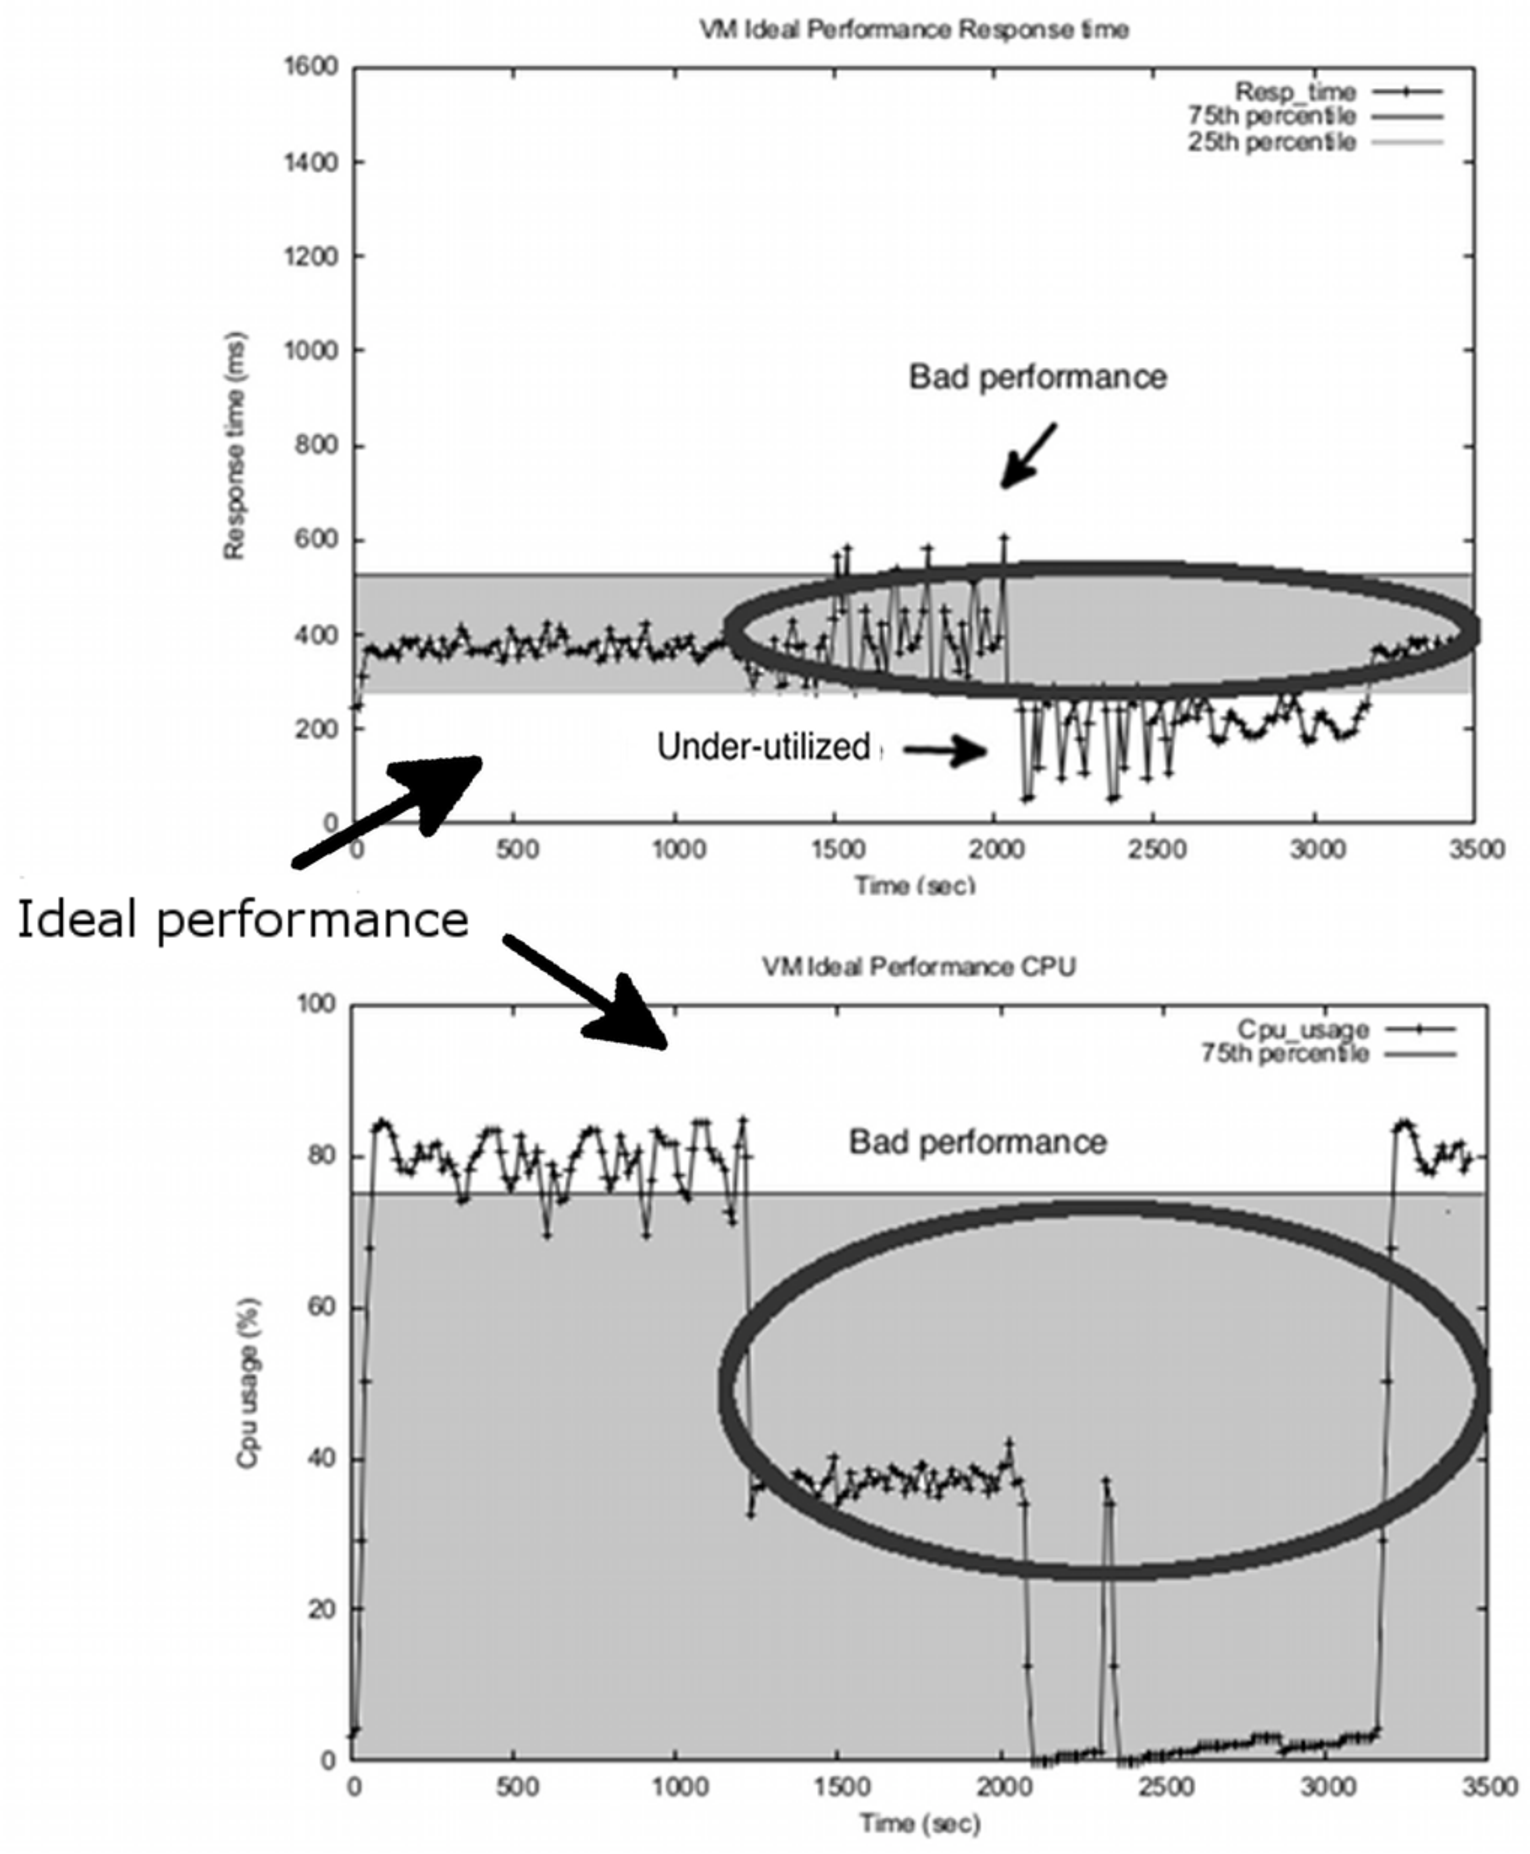
\includegraphics[width=\linewidth]{images/idealc1MediumRemark.pdf}
  \end{center}
  \caption{Profiling data and percentiles of c1.medium.}
  \label{fig:vm_performance2}
\end{figure}

%\begin{figure*}[htb]
%	\begin{minipage}[b]{0.45\linewidth}
%		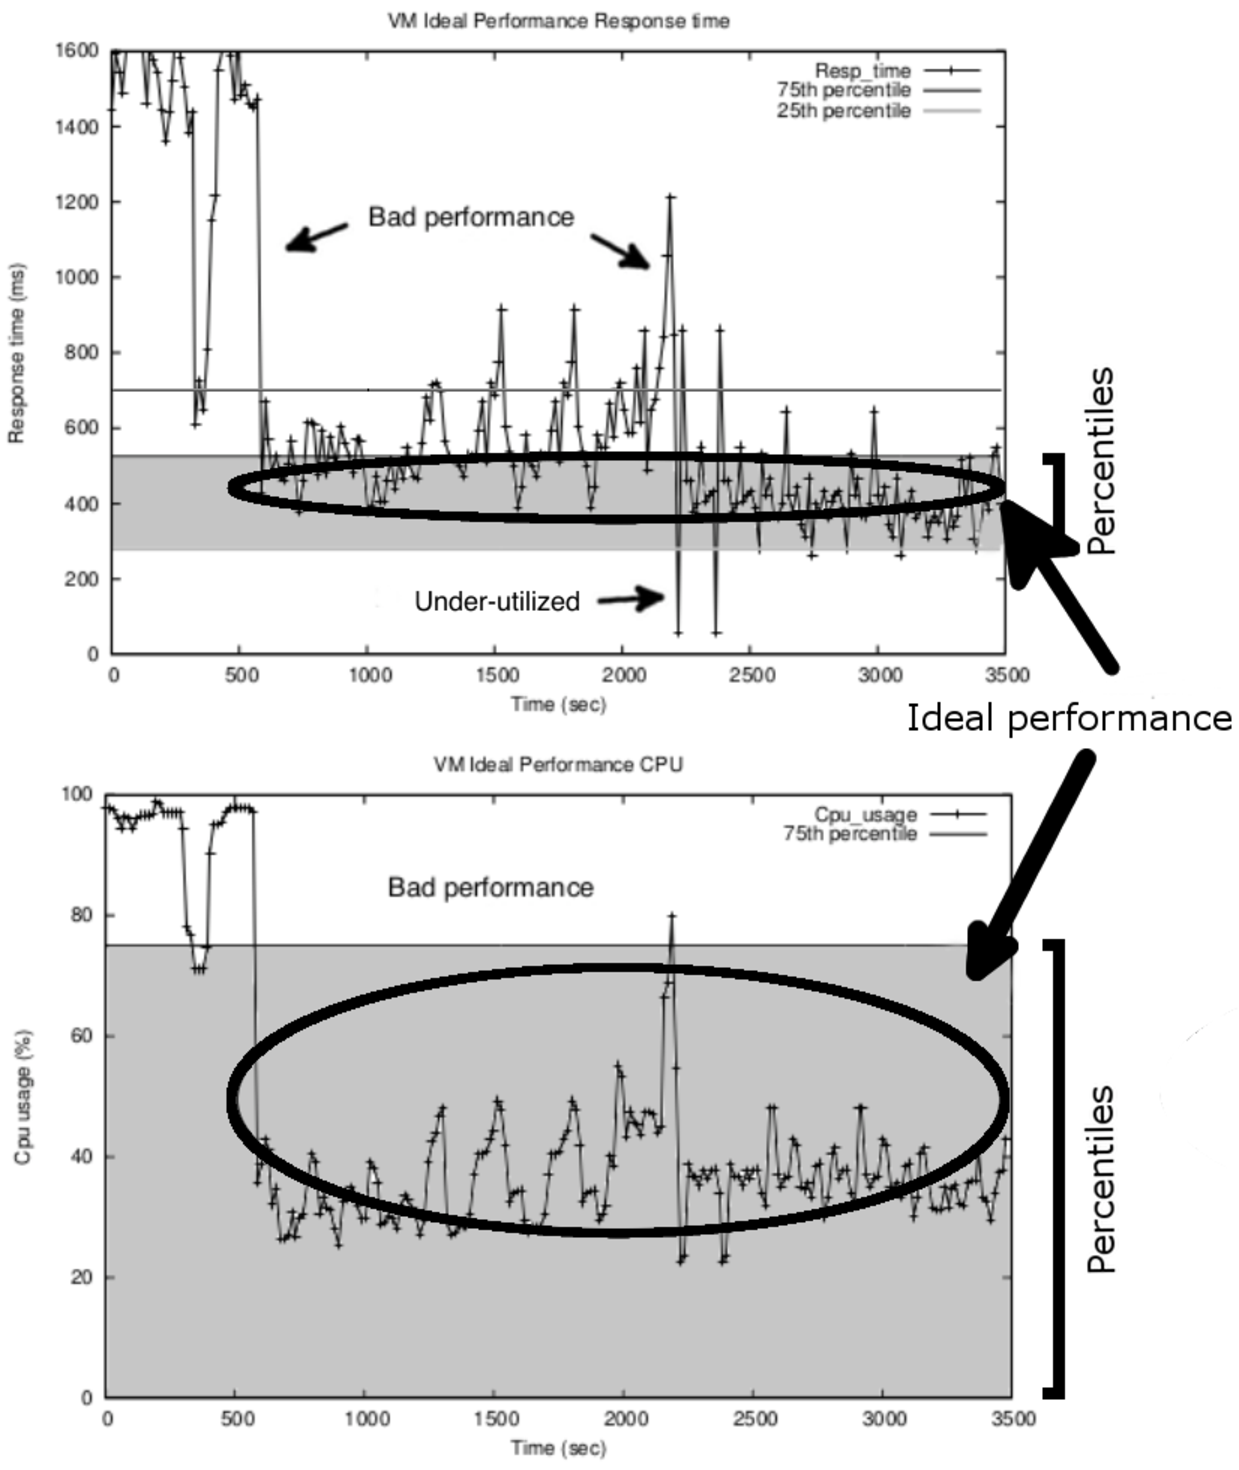
\includegraphics[height=8.5cm]{images/idealSmallRemark.pdf}		
%		\captionof*{figure}{ \textbf{m1.small}}	
%		\vspace{-4mm}
%	\end{minipage}
%	\hfill
%	\begin{minipage}[b]{0.45\linewidth}
%		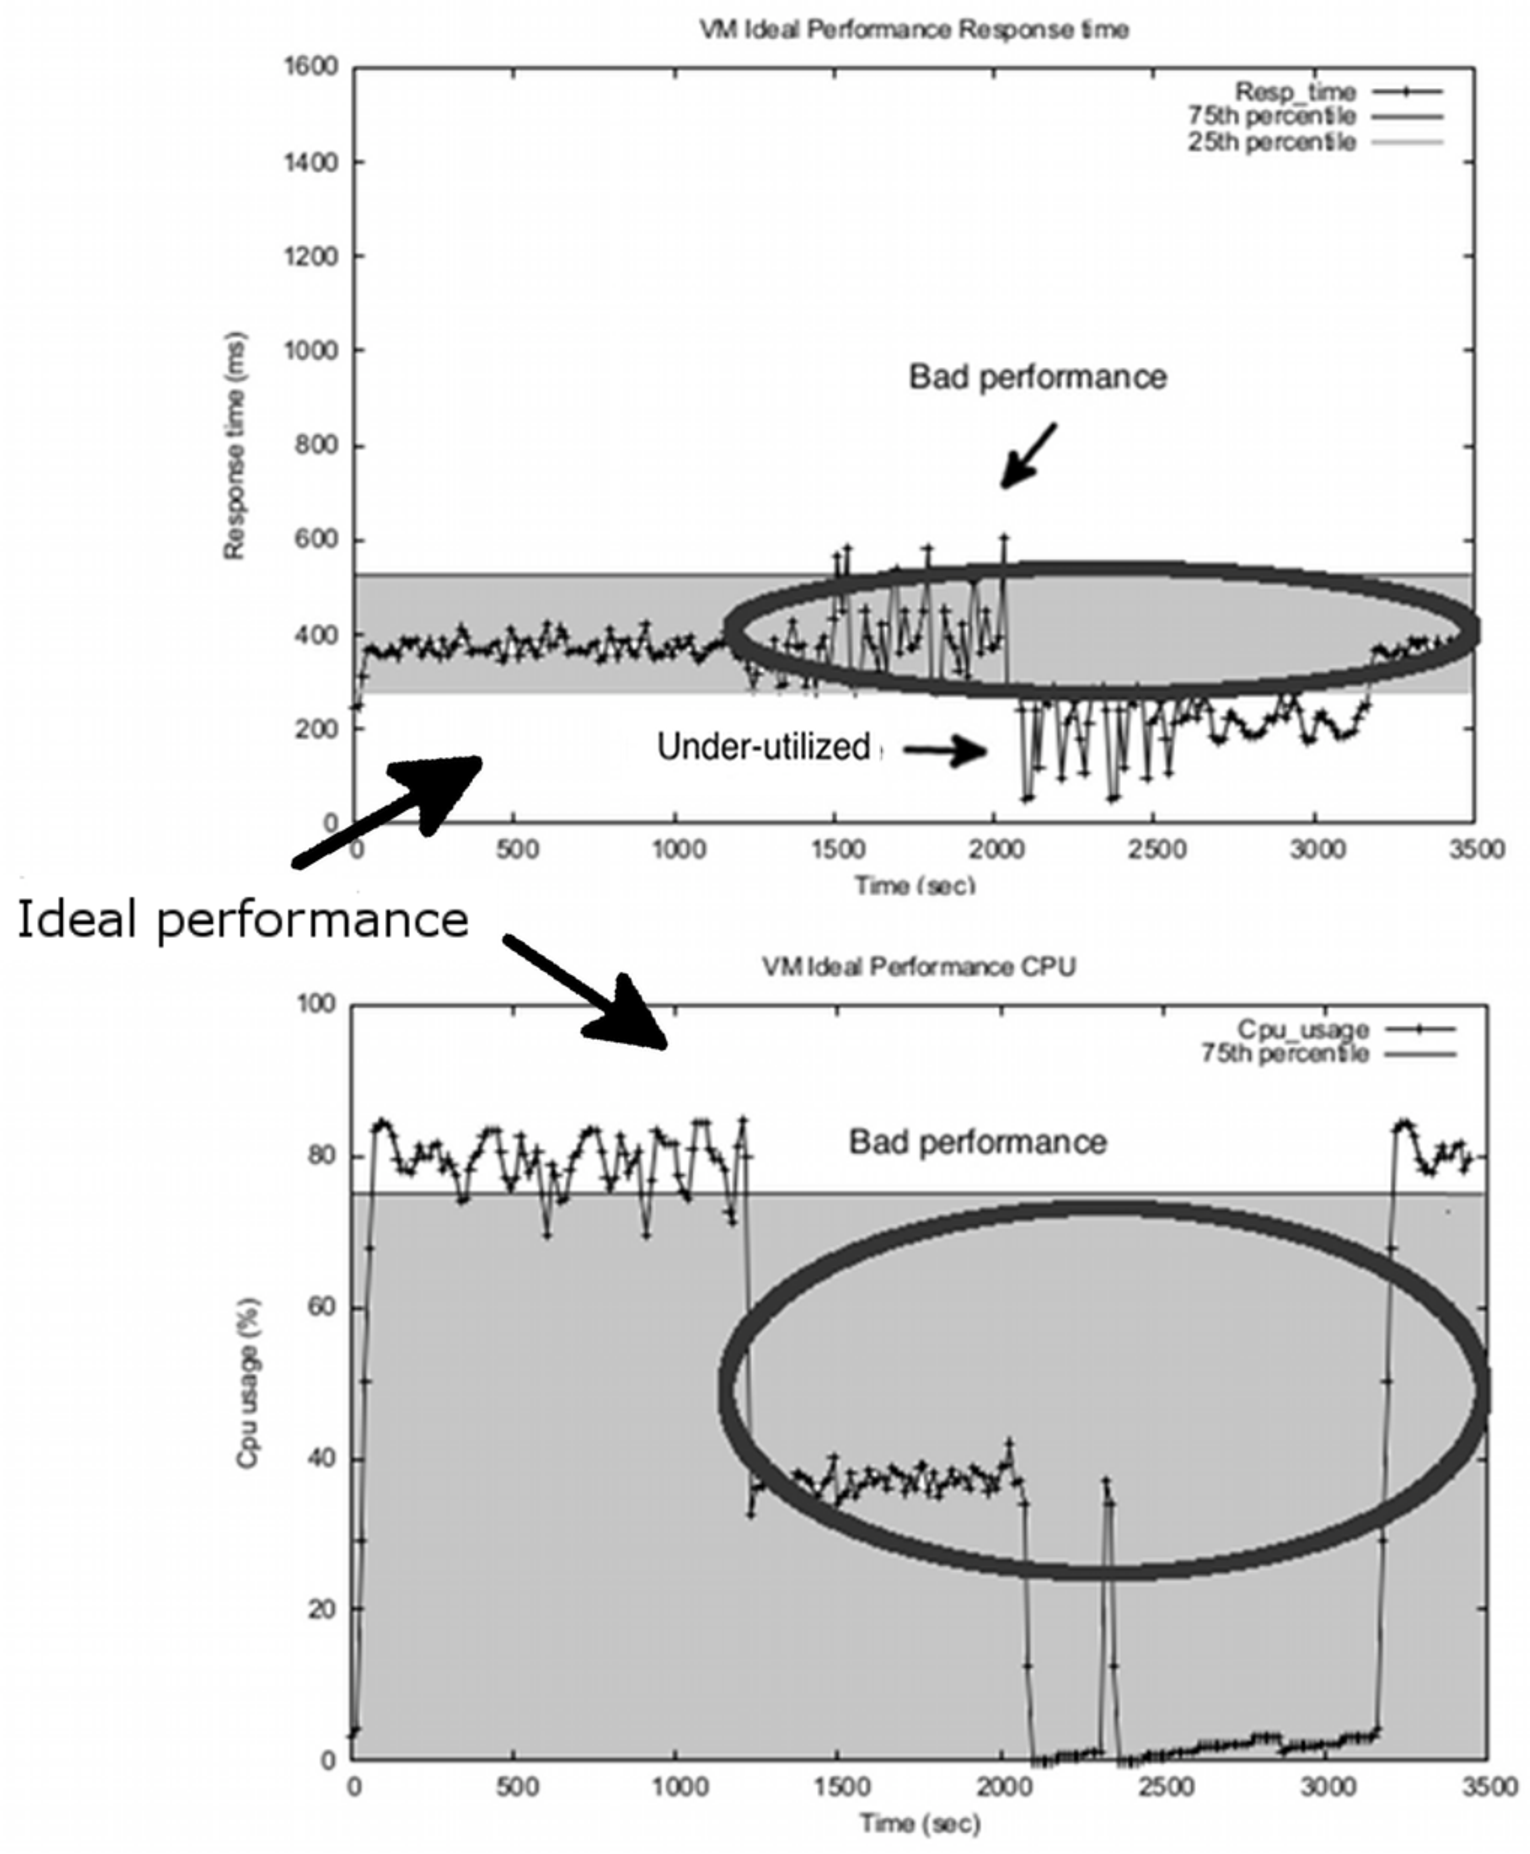
\includegraphics[height=8cm]{images/idealc1MediumRemark.pdf}
%		\captionof*{figure}{ \textbf{c1.medium}}
%		\vspace{-4mm}
%	\end{minipage}
%\caption{Profiling data and percentiles of m1.small and c1.medium EC2 instances.}
%\label{fig:vm_performance}
%\end{figure*}

\item Classify the different instance types depending on its computing capacity. Using the profiling smoothed data of each instance type (refer to Lines \ref{alg:throughput_start}-\ref{alg:throughput_end}), the Profiler computes a factor, named \emph{Ideal\_Throughput$_{inst}$}, as the amount of clocks required to serve a specific amount of requests (clocks/requests)  for one instance. In Equation~\ref{cpu_speed}, the \emph{\%CPU\_usage$_{inst}$} represents the average of percentage of cpu usage (clocks) and \emph{Num\_requests$_{inst}$} the average of request rate (requests) consumed during the last hour.

\fixme{Explain how we get the cpu usage.}


{\scriptsize
\begin{equation}\label{cpu_speed}
\begin{split}
\% CPU\_usage_{inst} = \dfrac{   \sum_{i=1}^N \big( \% cpu\_usage\_data_{i}  \big) } { N } \\
Num\_requests_{inst} = \dfrac{   \sum_{i=1}^N \big( req\_rate\_data_{i} \big) } { N } \\
Ideal\_Throughput_{inst} =\dfrac{ \bigg( \dfrac{\% CPU\_usage_{inst} } { 100 }  \bigg) } {  Num\_requests_{inst}   } 
\end{split}
\end{equation}
}

The \emph{Ideal\_Throughput$_{inst}$} factor gives an estimation of the optimized performance capacity of one VM instance when processing the current workload. Based on the value of this factor per-instance, the \emph{Profiler} classifies the different instance-types based on its computing capacity when running an application. (See Lines \ref{alg:clas}-\ref{alg:end_clas}). The resulting classification gives an interesting feedback to the Scaler component, which is now able to identify the capacity of each instance type, and consequently to choose an optimal scaling plan. Note that, a lower value of the \emph{Ideal\_Throughput$_{inst}$} indicates a higher performance capacity. Initially, there are not instance profiles due to the lack of monitoring data, thereby the \emph{Scaler} uses the number of compute units per instance as a priori classification of their performance capacities. This work only consider the compute units, but memory or bandwidth can be also taken into consideration to classify the VM instances.
\end{enumerate}

This profiling process allows to define a profile per instance type, thus facilitating the selection of an appropriate scaling plan that will satisfy the QoS requirements. Similarly, the profiling data can be used independently of factors such as performance isolation in clouds or request heterogeneity to improve the accuracy of the scaling decisions. Even though this profiling approach assumes that all the resources of the same type behave similarly, it can be easily extended to profile the allocated resources independently of its type. The performance of VM instances provided by current clouds is largely heterogeneous, even among instances of the same type~\cite{ec2Performance}.



\subsection{Scaling plan decision-making}

The discovery of a proper scaling plan is the most important and challenging phase in a provisioning system. It is responsible of the selection of an appropriate combination of resources that fulfills the QoS requirements.
% with the lowest operational cost. 

%This operation can become more laborious when running web applications, and therefore it has been barely addressed in the existing provisioning systems. Web applications are often a target of temporal traffic variations that may cause SLO violations having an impact in the user experience. Hence, the selection of an appropriate scaling plan becomes crucial to mitigate these penalties. 

%On the other hand, to boost the volume of customers, the user experience appears as a mandatory requirement in web applications contrary to budget cuts that may reduce the advantage over competitors.

To overcome this task, we should take into consideration three aspects: the workload requirements, the resource heterogeneity and the customer preferences. An exhaustive analysis of the current workload allows to identify the future demand that will determine the new configuration to use. This operation can become more laborious when running web applications due to their workload heterogeneity. On the other hand, cloud infrastructures offer a wide range of different hardware configurations that can be combined to better satisfy the requirements. Based on the customer preferences, the selection of one configuration or another can expose the application to availability or performance issues, specifically when handling workload variations or other traffic anomalies. Hence, the selection of an appropriate scaling plan becomes crucial to mitigate these penalties. 

%% Threshold fixed by the user



%\begin{figure*}[htb]
%	\begin{minipage}[b]{0.3\linewidth}
%		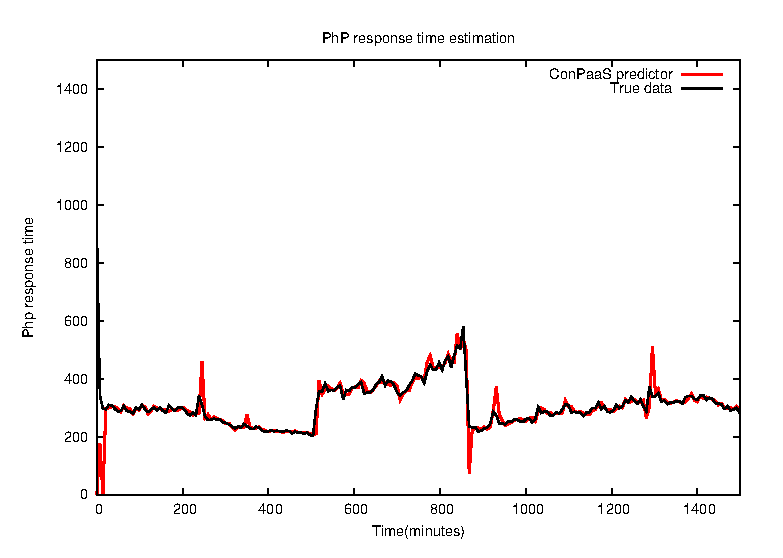
\includegraphics[height=4.5cm]{images/prediction_conpaas_6min.eps}
%		\vspace{-4mm}
%	\end{minipage}
%	\hfill
%	\begin{minipage}[b]{0.3\linewidth}
%		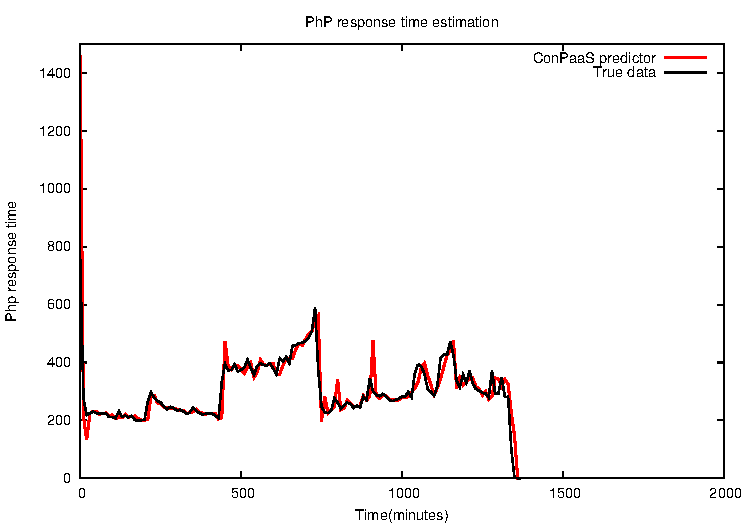
\includegraphics[height=4.5cm]{images/prediction_conpaas_10min}
%		\vspace{-4mm}
%	\end{minipage}
%	\hfill
%	\begin{minipage}[b]{0.3\linewidth}
%		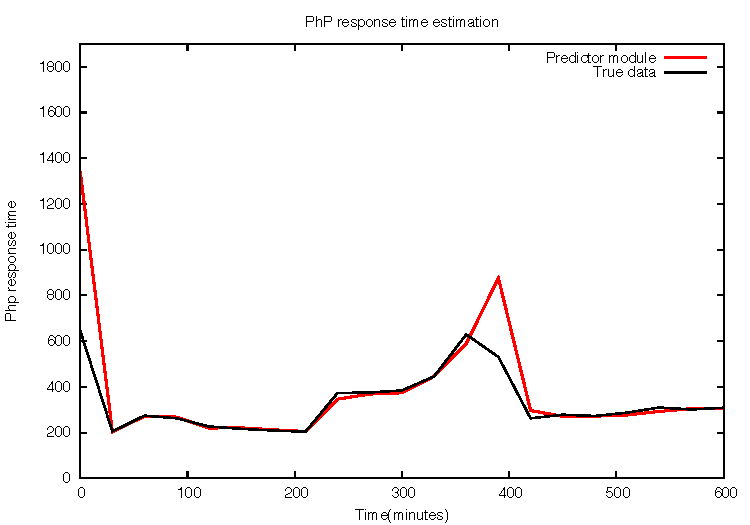
\includegraphics[height=4.5cm]{images/prediction_conpaas_30min}
%		\vspace{-4mm}
%	\end{minipage}
%\caption{ConPaaS Predictions, response times for 5min, 10min and 30min ahead.}
%\label{fig:vm_performance}
%\end{figure*}

%\subsubsection{Scaling strategy decision-making}



\subsubsection{Analysis of the workload requirements}

Prior to any resource selection, the \emph{Scaler} has to measure the requirements of the current workload taken into account the traffic diversity of web applications. Traditional scaling systems gather monitoring data about the request volume or total percentage of cpu usage consumed to identify the workload requirements. However, the workload of web applications is highly heterogeneous being defined by sudden changes in the traffic as well as constantly-changing request mixes. As a consequence, our system computes the workload complexity considering both the total percentage of cpu usage and request rate served by the current scaling plan,  as factors that affect to the final response time. They provide enough information to detect the causes of a performance degradation in web applications. 

%In Equation~\ref{workload_complexity}, the \emph{$Workload_{complex}$} factor represents the complexity of the incoming traffic and includes degradations caused by operative system activities, low network performance, performance isolation or request heterogeneity. These degradations are omitted by individually analyzing the request rate or cpu usage consumed by all the allocated resources at any given time. Thus, the \emph{$Workload_{complex}$} is computed by using the sum of the cpu usage (denoted by \emph{$CPU\_usage_{i}$}) and the performance capacity of each allocated resource. The performance capacity is calculated as the average of the request rate served by each resource (denoted by $Num\_reqs_{i}$) and its ideal throughput (denoted by $Ideal\_Throughput_{inst_{i}}$). By using the ideal throughput instead of calculating the current throughput, the Scaler is able to measure how much the current workload is affecting the ideal performance pattern of a VM instance.

The \emph{workload complexity} is a factor that identifies how much the current workload is affecting the ideal performance pattern of the allocated resources. It identifies the complexity of the incoming traffic and includes degradations caused by operating system activities, low network performance, performance isolation or request heterogeneity. These degradations affect the performance and are often omitted by individually analyzing the request rate or cpu usage consumed by the allocated resources. 

To calculate the \emph{workload complexity} (denoted by \emph{$Workload_{complex}$}), we first analyzes the monitoring data gathering the request rate (denoted by $Num\_reqs\_server_{i}$) and total percentage of cpu usage (denoted by \emph{$\%CPU\_usage\_server_{i}$}) consumed by the allocated \emph{N} resources during the monitoring window. Secondly, unlike the \emph{\%CPU\_usage$_{inst}$},  we calculate the expected cpu usage of each resource \emph{i} (denoted by \emph{CPU\_usage\_expected$_{i}$} ) using its current request rate (denoted by $Num\_reqs\_server_{i}$) and its \emph{optimized throughput} (denoted by $Ideal\_Throughput_{inst_{i}}$). By doing so, we are able to include into the \emph{$Workload_{complex}$} all the degradations that affect the ideal performance of the application. Finally we compute the \emph{$Workload_{complex}$} factor using the sum of cpu usage consumed to handle the current workload and the sum of expected cpu usage of all the resources, as illustrated in Equation~\ref{workload_complexity}.


%\fixme{We could include in the Equation some additional information to define each factor.}

{\scriptsize
\begin{equation}\label{workload_complexity}
\begin{split}
CPU\_usage\_expected_{i} =  Num\_reqs\_server_{i}  * Ideal\_Throughput_{inst_{i}} \\
Workload_{complex}  = \dfrac{ \bigg(  \dfrac{ \sum_{i=1}^N \%CPU\_usage\_server_{i} } {100} \bigg) }  {  \sum_{i=1}^N  CPU\_usage\_expected_{i}     } = \dfrac{ \ (clocks) }  {  (clocks) }
\end{split}
\end{equation}
}

Additionally, the future service demand of the application, in terms of total percentage of cpu usage and request rate consumed by the resources, can be estimated by the \emph{Predictor} component for the next monitoring windows (in our experiments 30min). This enables to select in advance a scaling strategy that will handle future fluctuations in the workload, and thereby saving cost. As an example in Figure~\ref{fig:forecast}, the \emph{Predictor} shows the forecast values for the resource requirements during the next 30 minutes offering an acceptable level of accuracy. To calculate the precision of the forecasting results, we used metrics such as PRED(25)~\cite{jorgensen_experience_1995} and Mean Absolute Percentage Error (MAPE)~\cite{islam_empirical_2012} that obtained values 0.904 and 0.109 respectively. By definition, PRED(25) values closer to 1.0 and MAPE values closer to 0.0 indicates a better fit of the prediction model; thus indicating correct prediction rate of our forecasting results.

% An aspect to notice is that the forecasting results never under-provision the system avoiding the generation of unnecessary SLO violations.

% PRED(25) value closer to 1.0 indicates a better fit of the prediction model.
% A lower value of MAPE implies a better fit of the predciction model; thus indicating superior prediction accuracy.
% PRED(25) = num. observations with relative error <= 25% / num observations = 19/21 ... and MAPE = 1/n sum( |y_pred - y| /y )

\begin{figure}[t]
  \begin{center}
    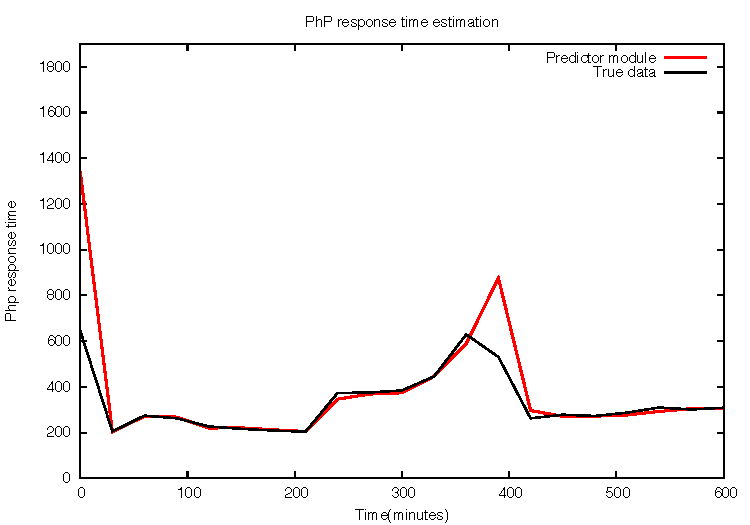
\includegraphics[width=\linewidth,height=6cm]{images/prediction_conpaas_30min}
  \end{center}
  \caption{Predictor component: forecasting results for 30min ahead.}
  \label{fig:forecast}
\end{figure}


\subsubsection{Calculating the different scaling plans}

To decide which type and amount of VM instances to add or release, the \emph{Scaler} uses an optimal decision tree that facilitates the discovery of all the possible scaling strategies. By going through this tree, our system evaluates all the possible resource combinations using horizontal scaling operations (out, back). As shown by Figure~\ref{fig:scalingTree}, in the scaling decision tree, each node represents each type of hardware configuration offered by a cloud infrastructure, where the nodes linked by a straight line represent the current scaling strategy. While the branches, denoted by a dotted line, define all the possible resource combinations to provision. 

\begin{figure}[t]
  \begin{center}
    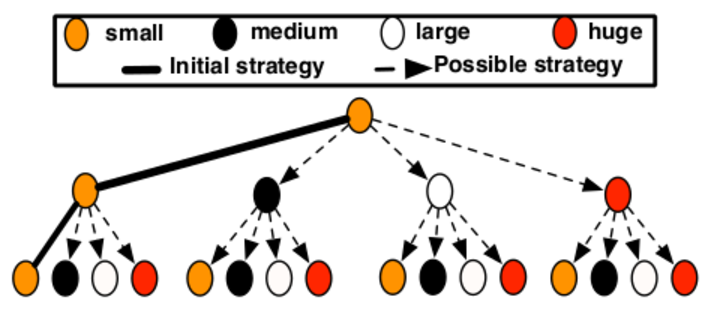
\includegraphics[width=0.85\linewidth,height=4cm]{images/optimalTree_initial}
  \end{center}
  \caption{Example of a decision tree created from an existing resource combination.}
  \label{fig:scalingTree}
\end{figure}

During the selection process of possible scaling strategies, the \emph{Scaler} uses the Equation~\ref{resource_combination} to compute how a strategy will distribute the current workload across the different resources taken into account their performance capacities.  Equation~\ref{resource_combination} defines a factor, called \emph{RU\_Strategy}, that determines the resource utilization of a strategy when handling the current or future workload (depending on how the workload requirements were obtained). According to that, the \emph{Scaler} selects a strategy that uses \emph{N} resources to distribute the \emph{$Num\_reqs_{total}$} (total requests served by the current resources or estimated by the \emph{Predictor}) with a workload complexity \emph{$Workload_{complex}$} across \emph{N} instance types with different optimized throughputs \emph{$Ideal\_Throughput_{inst_{k}}$}. As a function of the \emph{$Ideal\_Throughput_{inst}$} and \emph{$Num\_reqs_{total}$}, the \emph{$RU\_Strategy$} measures the resource utilization (clocks) to process the current workload when using a specific resource combination.

%When processing the current workload, to decide which resources to include in the scaling plan,  the \emph{Scaler} uses the following formula: 

%This formula determines the CPU usage consumed to process the current workload when using a specific resource combination (denoted by \emph{$CPU_{strategy}$}). Note that, CPU usage provides enough feedback about the performance capacity, as it is a function of the request complexity  and number of served requests. 

%To calculate the different combinations of VM instances that enforce the performance requirements, we used the next

{\scriptsize
\begin{equation}\label{resource_combination}
\begin{split}
\text{RU\_Strategy = Resource utilization of the strategy} \\ \\
RU\_Strategy_{i} = \dfrac{ \sum_{k=1}^N \bigg( \bigg( \dfrac{ Num\_reqs_{total} } {N}  * Workload_{complex} \bigg) * Ideal\_Throughput_{inst_{k}} \bigg) }  {N} \\ 
%\\ {\small \textit{ If } CPU\_usage_{strategy} \leqslant CPU\_max_{SLO} }
\end{split}
\end{equation}
}



%As an example, Figure~\ref{fig:scalingTree} shows three scaling plans that propose three different resource combinations: (left) a strategy is selected by adding two new \emph{small} instances, (center) a strategy proposes to replace one \emph{small} instance by one \emph{large}, and (right) both operations are combined by replacing one \emph{small} instance by one \emph{medium} and then adding one \emph{small}. 

Note that, the search space of possible strategies can be as large as the number of available hardware configurations, and allocated resources of the current scaling plan. It makes hard-to-find the best resource combinations in a reasonable short period of time, so that the \emph{Scaler} filters the possible strategies based on the following criteria:

\begin{itemize}
\item Define the maximum resource utilization consumed  by a strategy when processing a particular workload (denoted by \emph{$Max\_RU\_Strategy$}). It limits the number of possible plans where \emph{$RU\_Strategy_{i} \leq Max\_RU\_Strategy$}. \emph{$Max\_RU\_Strategy$} specifies the maximum resource utilization at which the application starts to experience SLO violations or over-utilization of the resources. Its value can be extracted either from the Amazon EC2 recommendations for the maximum percentage of cpu usage (cpu usage always lower than 75\%), or based on the monitoring data at which the application starts to experience SLO violations. As a result of this policy, the proposed scaling plans optimizes the current performance below values causing performance degradations. 

%can be calculated either based on the Amazon EC2 recommendations ( CPU values always lower than 75\%), or based on the CPU values at which the application starts to experience SLO violations (or performance degradations). 

\item Include a cost policy to avoid choosing wasteful scaling strategies. Considering the pricing model of cloud providers that charges users on a per-hour basis, the \emph{Scaler} includes a cost policy that rejects strategies releasing resources which have been recently started ( 5min $<$ time to the end of its hour $<$ 20). The \emph{Scaler} releases resources which are closed to the hour are free under the cloud pricing model, and there is no gain from terminating them before this hour price boundary.

\end{itemize}

These two policies avoid to trigger new scaling actions in short time intervals (e.g. within less than one hour), and consequently reduce the operational cost. 


%As an example of the selection process
\noindent\textbf{Example:} Figure~\ref{fig:scalingTreeSelection} shows three possible scaling plans obtained by using our decision tree and Equation~\ref{resource_combination} (denoted by \emph{Eq(3)}) over the initial strategy illustrated in Figure~\ref{fig:scalingTree}. This initial resource combination is composed of three \emph{small} instance types which are not enough to handle the current workload. Using this strategy as reference and horizontal scaling operations, our algorithm adds and/or releases resources (leafs to the tree) as long as the resulting \emph{$RU\_Strategy$} (calculated for the new resource combination) is lower than \emph{$Max\_RU\_Strategy$} and do not propose to release resources recently added. As a result, three plans (trees) are proposed using different resource configurations and satisfying the performance requirements to handle the workload. This discovery process stops when all the possible combinations have been proved or there are not more combinations satisfying the aforementioned filtering criteria. 



\begin{figure}[t]
  \begin{center}
    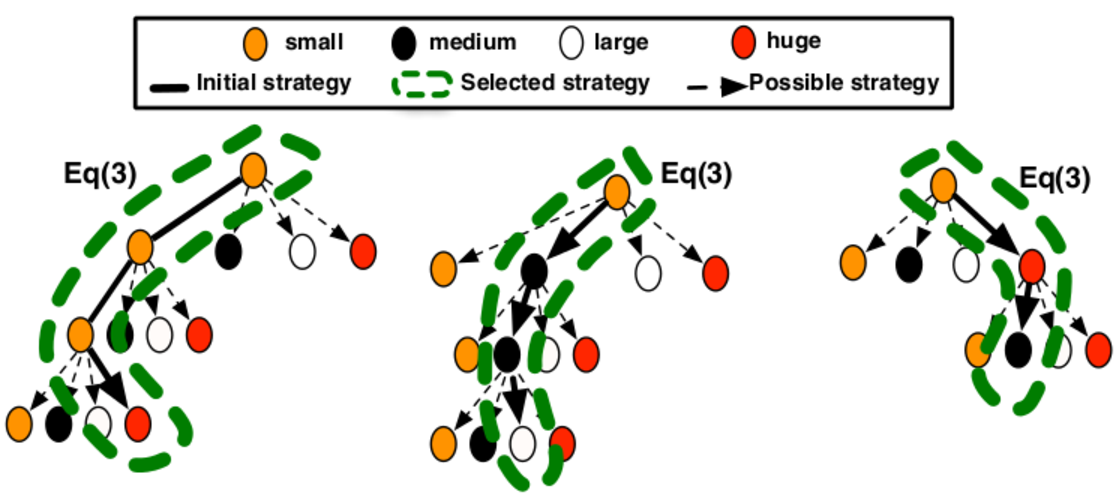
\includegraphics[width=\linewidth,height=4.5cm]{images/optimalTree_selection}
  \end{center}
  \caption{Example of three selected scaling plans that satisfy the filtering criteria.}
  \label{fig:scalingTreeSelection}
\end{figure}



In summary, using the Equation~\ref{resource_combination}, the Scaler is able to answer to the question \emph{"How many and which type of VM instances to provision?"}.

%is calculated using the Profiler component and will variate depending on the type of vm instance used in the strategy. 

\subsubsection{Selecting the optimal scaling plan}

%To refine this search process according to the final goal and adapted to the customer preferences (user experience), the Scaler provides three classes of SLA agreements in function of the type of customer. These three classes of customers namely, gold, silver and bronze minimize the SLA violations with a different infrastructure cost. Accordingly, a gold customer pays more in order to get the best service at the cost of some extra over-provisioning. A silver customer gets good availability while a bronze customer obtains a reduced, but acceptable, SLA fulfillment but with very little over-provisioning.

%they are classified based on their infrastructure cost and degree of SLO fulfillmen

Once the \emph{Scaler} obtains a list of filtered scaling strategies, it computes the cost of applying each possible strategy how the cost incurred by its SLO fulfillment degree and the infrastructure cost. The infrastructure cost (denoted by \emph{Infra\_cost}) specifies the cost required to provision a scaling plan for the next hour. While the SLO fulfillment degree (denoted by \emph{SLO\_fulfillment}) indicates the vulnerability of a scaling plan to experience SLO violations. 

As defined in the Equation~\ref{strategy_cost}, the \emph{SLO\_fulfillment} cost is calculated given the \emph{$RU\_Strategy_{i}$} of a strategy \emph{i} and the \emph{$Max\_RU\_Strategy$}. Obviously, higher values in the \emph{$RU\_Strategy$} imply an increment in the probability of having SLO violations under traffic spikes, so the \emph{SLO\_fulfillment} will increase as well. 

%As defined in the Equation~\ref{strategy_cost}, the \emph{slo\_fulfillment} cost is calculated given the percentage of \emph{$CPU_{strategy}$} and the \emph{$CPU_{SLO}$}, multiply by a SLO penalty (in \$)  pre-established between the customer and provider. Obviously, higher values in the percentage of \emph{$CPU_{strategy}$} imply an increment in the probability of having SLO violations under traffic spikes, so the \emph{slo\_fulfillment} will increase as well. 

%Therefore, according to the customer preferences, the Scaler can select one strategy with the lowest, highest or medium cost.

{\scriptsize
\begin{equation}\label{strategy_cost}
\begin{split}
Infra\_cost_{i} = \sum_{k=1}^N \big( instance\_price_{k} \big) \\
%slo\_fulfillment =  \bigg( \dfrac{ CPU_{strategy} } {CPU_{SLO}} \bigg) * SLO penalty \\
SLO\_fulfillment_{i} =  \bigg( \dfrac{ RU\_Strategy_{i} } {Max\_RU\_Strategy} \bigg)  \\
Cost\_strategy_{i} = \dfrac{  SLO\_fulfillment_{i}  } {Infra\_cost_{i}}
\end{split}
\end{equation}
}

%\fixme{I could omit the use of the SLO penalty, as it is a constant in my experiments. Instead I could say that the system adapts to the user needs.}

The criteria for the selection of the optimal scaling plan is configurable, and thereby it can adapted to the customer preferences. For instance, large enterprises need to provide high availability and performance to their clients, disposing of a generous budget for such a mission. Therefore, based on the customer-tradeoff between performance/cost, the \emph{Scaler} component will choose to provision one scaling plan or another depending on the value of its \emph{Cost\_strategy}. 

To facilitate the specification of the performance/cost preferences to the customers, our system provides different pre-defined criteria that adapt the scaling decisions to these requirements. These selection criteria are defined thanks to a \emph{metal classification} that classifies  the different type of customers based on their performance/cost preferences. Initially, we define three different classes of customers following this \emph{metal classification}. These three classes of customers namely, Gold, Silver and Bronze minimize the SLA violations with a different infrastructure cost. 

\begin{itemize}
\item A \emph{Gold customer} identifies those customers that pay more in order to get the best service at the cost of some extra over-provisioning. 
\item A \emph{Silver customer} includes those customers that prefer to get good availability but with a reasonable operational cost.
\item A  \emph{Bronze customer} represents those customers who are willing to obtain a reduced, but acceptable, SLO fulfillment but with very little over-provisioning; and thereby a low operational cost. 

\end{itemize}

In our experiments, we will use this \emph{metal classification} to show the benefits/drawbacks by selecting different scaling plans based on the class of customer.
% when handling sudden workload variations.

%To classify the provisioning decisions based on the tradeoff between performance/cost of the customer preferences, we define three different classes of customers following a medal classification. These three classes of customers namely, gold, silver and bronze minimize the SLA violations with a different infrastructure cost. For instance, a gold customer pays more in order to get the best service at the cost of some extra over-provisioning. A silver customer gets good availability while a bronze customer obtains a reduced, but acceptable, SLO fulfillment but with very little over-provisioning. 



%Moreover, \emph{$SLO_{penalty}$} can be also used as a criteria for the selection of the most appropriated strategy according to some requirements.

%To decide which type of instance to release, the Scaler uses a conservative algorithm that releases the resources with the lowest utilization by analyzing their monitoring data. Similarly, a cost policy was also included for avoiding to choose wasteful scaling decisions. Considering the pricing model of cloud providers that charges users on a per-hour basis, the Scaler includes a cost policy that rejects strategies releasing vm instances which have been recently started ( 5min < time to the end of its hour < 20). Scaler releases resources which are closed to the hour are free under the cloud pricing model, and there is no gain from terminating them before this hour price boundary.

%A complete point of view of the whole scaling flow is shown in Figure~\ref{autoScalingFlow}.

%\begin{figure}[htb]
%  \begin{center}
 %   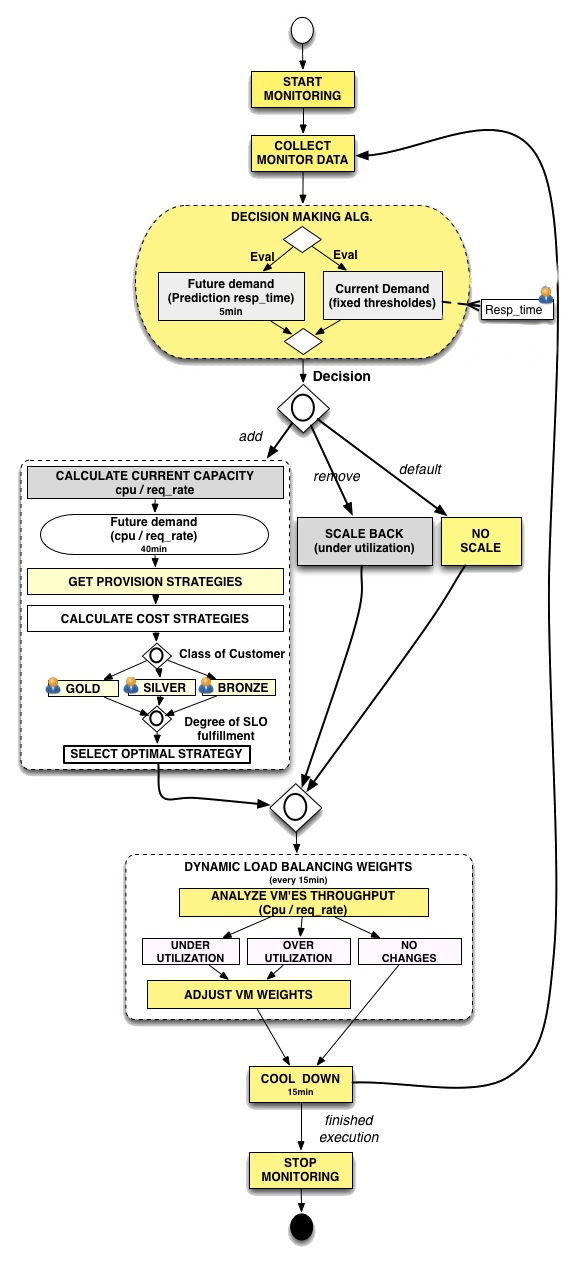
\includegraphics[width=\linewidth]{images/NewAutoScalingFlow}
%  \end{center}
%\vspace{-5mm}
%  \caption{Auto scaling flow.}
%  \label{autoScalingFlow}
%\end{figure}


\subsection{Dynamic load balancing weights } 


The problem we consider here is again the heterogeneity of cloud platforms.
Independently of its size, different VM instances from the same cloud might have different performance
characteristics, even when their specifications from the cloud vendor are 
the same~\cite{ec2Performance}. This issue can be addressed through various 
load balancing techniques, like assigning weights to the backend servers or 
taking into account the current number of connections that each server 
handles. Furthermore, the performance behavior of the virtual servers may 
also fluctuate, either due to changes in the application's usage 
patterns, or due to changes related to the hosting of the virtual servers 
(e.g., VM migration).


\begin{figure}[t]
  \begin{center}
    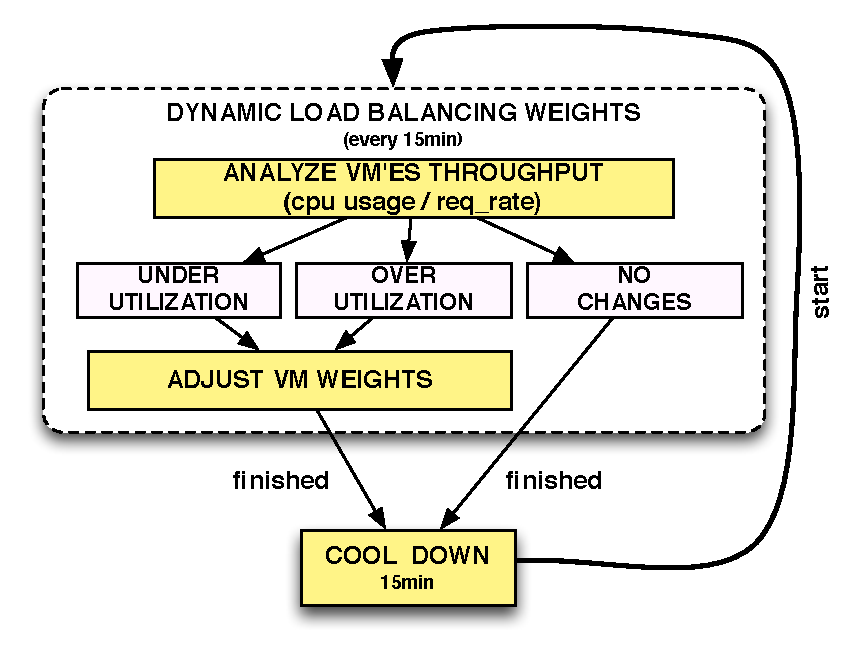
\includegraphics[height=5cm]{images/load_balancing}
  \end{center}
  \caption{Weighted load balancing flow.}
  \label{fig:load_balancing}
\end{figure}


In order to address these issues, the Scaler implemented a weighted 
load balancing system in which the weights of the servers are 
periodically re-adjusted automatically, based on the monitoring data.  
This method assigns the same weight to each backend server at the 
beginning of the process. As illustrated in Figure~\ref{fig:load_balancing}, the weights are then periodically
adjusted (in our experiments, using a window of $\sim$ 15min) proportionally 
with the difference among the average of percentage of cpu usage and request rate served by the servers 
during this time interval. By adding this technique to our autoscaling system, 
the workload can be dynamically and proportionally distributed across the provisioned VM instances depending on their performance capacities.

%we noticed a performance improvement when running the benchmarks, as discussed in the following.





\section{Evaluation}
\label{sec:evaluation}
To compare the provisioning algorithms described above, we ran experiments
on two infrastructures: a homogeneous one (the DAS-4, a multi-cluster system
hosted by universities in The Netherlands~\cite{das4}) and a heterogeneous
one (the Amazon EC2 cloud~\cite{amazonEC2}). The goal of our experiments
was to compare the algorithms by how well they fulfill the SLOs and by
the amount of resources they allocate.

%In this section we conducted our experiments on a heterogeneous infrastructure like Amazon EC2~\cite{amazonEC2}, and on a homogeneous infrastructure like DAS-4 (the Distributed ASCI Supercomputer 4)~\cite{das4}. In our experiment campaign, we compared the degree of SLO enforcement and resource consumption for each provisioning algorithm implemented in ConPaaS. 

%DAS-4 is the Dutch Computational Infrastructure, a six-cluster wide-area distributed system designed with research purposes

\textbf{Testbed configuration:}  As a representative scenario, we deployed the MediaWiki application using ConPaaS on both infrastructures, and we ran the Wikibench tools with a 10\% sample of a real Wikipedia access trace for 24hours. 
%Consequently, our goal is to evaluate the behavior of the provisioning algorithms, when scaling out and back the number of VMs hosting PhP servers to guarantee several performance requirements, referred to as SLO.  Accordingly, some assumptions were made:
We configured the experiments as follows: 

\begin{itemize}
%\item  Response times from static requests were not analyzed due to its lightweight nature. 

\item The monitoring data was collected over a reporting period of 5 minutes.

\item We fixed a SLO of 700 milliseconds at the service's side (denoted by a red Line on Figures~\ref{naiveDas4},\ref{historyDas4},\ref{naiveEC2},\ref{historyEC2}).


\item The dynamic load-balancing weights provisioning technique was only evaluated on the heterogeneous platform, Amazon EC2. This algorithm brings improvements to the feedback algorithm only in environments where VMs may have different hardware configurations. 

\item The algorithms used the same statistically-chosen performance threshold ranges. 

%\item A minimum interval of 15 minutes has been established between scaling actions to avoid excessive oscillations. 
\end{itemize}


%To provide the Wikipedia services, an initial configuration was composed of 4 VMs, and 1 VM to host the Wikibench tools. The 4 VMs include a PhP service manager VM, a PhP agent VM, a web server and a http-proxy agent VM (both in the same VM), and finally a MySQL agent VM to store the English Wikipedia data, as explained in Section~\ref{wikipedia}.

\subsection*{Homogeneous Infrastructure}

Our experiments on DAS-4 rely on OpenNebula as IaaS~\cite{sotomayor_virtual_2009}. To deploy the Wikipedia services, we used small instances for the PHP service (manager and agents) and a medium instance for the MySQL service (agent). In DAS-4, OpenNebula's small instances are VMs equipped with 1 CPU of 2Ghz, and 1GiB of memory, while medium instances are equipped with 4 CPU's of 2Ghz, and 4GiB of memory.

\paragraph{SLO enforcement.}
Figure~\ref{naiveDas4} and Figure~\ref{historyDas4} represent the degree of SLO fulfillment of the trigger-based and feedback algorithms, indicating the average of response times obtained during the execution of the Wikipedia workload trace. The results from Figure~\ref{naiveDas4} show that the trigger-based provisioning algorithm provokes an important amount of SLO violations at certain moments in time, due to its excessively reactive behavior. As we mentioned, this algorithm fails easily during traffic spikes, as it adds or removes VMs without evaluating the workload trend. The feedback algorithm, as shown on Figure~\ref{historyDas4}, handles the traffic spikes better and can achieve fewer SLO violations; specifically, there were 31.72\% less SLO violations in comparison with the trigger-based algorithm. 


\begin{figure}

\begin{center}
\includegraphics[width=0.49\textwidth, height=6cm]{./images/homogeneous/avgTimeout_PhP_trigger}
\end{center}
\vspace{-5mm}
\caption{Response time on DAS4 -- Trigger-based.}
\label{naiveDas4}
\end{figure}

\paragraph{Resource consumption.}

To better understand the behavior of both algorithms, we shall also focus on the resource consumption illustrated on Figure~\ref{resComDas4}. The excessively reactive behavior of the trigger-based algorithm can be noticed in the time intervals around \emph{t=350min} and \emph{t=820min}, where two scaling operations under-provision the system during a short period of time. These provisioning decisions provoked the SLO violations that are visible in Figure~\ref{naiveDas4}in the same intervals of time. Besides affecting the system's stability, such short fluctuations in the number of provisioned resource also raise the cost of hosting the application since more VM instantiations will be triggered. When using the feedback algorithm, the system makes provisioning decisions by analyzing the workload's trend. Scaling actions are only triggered when having \emph{constant} alterations in the workload, thereby providing a more efficient resource usage. We can see that the provisioning decisions made by the feedback algorithm on Figure~\ref{resComDas4} match well with the workload alterations depicted on Figure~\ref{workload}.

\begin{figure}
\begin{center}
\includegraphics[width=0.49\textwidth, height=6cm]{./images/homogeneous/avgTimeout_PhP_feedback}
\end{center}
\vspace{-5mm}
\caption{Response time on DAS4 -- Feedback.}
\label{historyDas4}
\end{figure}

\begin{figure}
\begin{center}
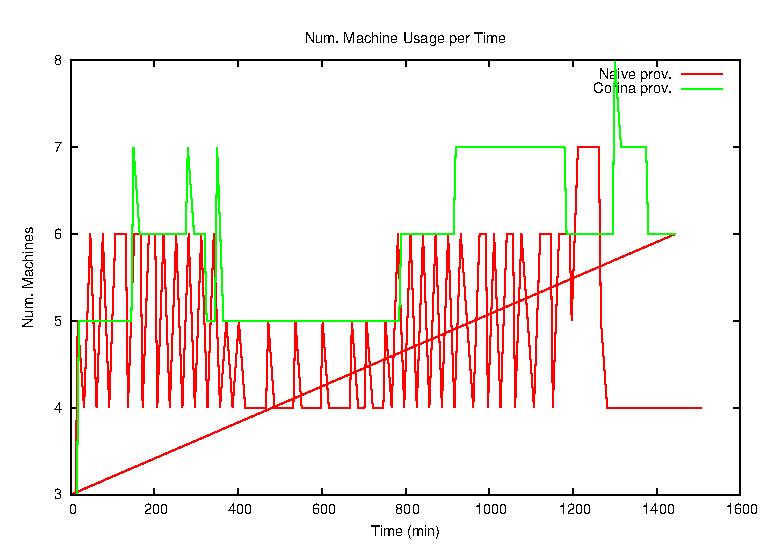
\includegraphics[width=0.49\textwidth, height=5cm]{./images/homogeneous/numMachinesComp}
\end{center}
\vspace{-5mm}
\caption{Resource consumption on DAS4.}
\label{resComDas4}
\end{figure}

\paragraph{Discussion.}

%Using the trigger-based provisioning algorithm, the system performance fluctuates greatly following a pattern similar to the web traffic, that increases the amount of SLO violations. The reactive behavior of this algorithm triggers scaling actions that affect to the system performance instead of improving it, and as a consequence, it is also wasteful in terms of resource consumption. Unlike feedback algorithm offers an efficient resource usage and a constant performance behavior while meeting the application's SLO. 

%Therefore this algorithm finds the trade-off between accuracy and cost savings.

%Both algorithms are best-effort regarding the SLO fulfillment, and thereby temporal alterations of the workload (with a short duration of 5min approx.) cannot be handled. The heterogeneity of the PhP-requests including images and requiring multiple Db queries, as well as the startup time of VMs (2-5min), are in part responsible of these SLO violations. 

Both algorithms are best-effort regarding the SLO fulfillment, and thus they do not handle well short alterations of the workload (with duration in the range of minutes). The heterogeneity of the PHP requests, as well as the startup time of VMs (2-5min), are in part responsible of these SLO violations.

%It avoid to under-provisioning in two occasions  while decreases the number of SLA violation. However, the naive alg. is vulnerable to temporal bursty workload variations (10 min), an increment of SLA violated is caused by under-provisioning operations in conjunction with workload variations. 



\subsection*{Heterogeneous Infrastructure}

Our experiments on EC2 used small instances for the PHP service (manager and agents) and  a medium instance for the MySQL service (agent). EC2 small instance are equipped with 1 EC2 CPU, and 1.7GiB of memory, while medium instances are equipped with 2 EC2 CPU's, and 3.75GiB of memory.

%In the following, we analyze the behavior of our algorithms when making provisioning decisions on a heterogeneous infrastructure.

\paragraph{SLO enforcement.}
Figure~\ref{naiveEC2}, Figure~\ref{historyEC2} and Figure~\ref{historyWeightEC2} show the system performance of the trigger-based, feedback and dynamic load-balancing weights algorithms, respectively. As depicted on Figure~\ref{naiveEC2}, the performance of the trigger-based algorithm is even more unstable than in the case of the homogeneous infrastructure. Two of the three peaks in response time, at \emph{t=300min} and \emph{t=820min}, can be explained by the variations in the Wikipedia workload shown in Figure~\ref{workload}. However, there is a third peak between \emph{t=400min} and \emph{t=500min} that corresponds to an interval of time in which the workload trace shows a significant drop in the request volumes. During this period of time, the algorithm attempts to scale down the system but the new lower number of resources cannot handle the load, and the system is scaled up again. As this algorithm does not keep any history information, after a short time it attempts again to scale down the system, with the same result; thus, some oscillations occur in the number of allocated resurces, causing also SLO violations.   

Figure~\ref{historyEC2} and Figure~\ref{historyWeightEC2} show that the
feedback and dynamic load-balancing algorithm reduce the number of SLO 
violations and provide a more stable performance pattern. Specifically,
with the feedback algorithm  we obtained 41.3\% less SLO violations than
with the trigger-based algorithm, while the dynamic load balancing algorithm
had 47.6\% less violations than the trigger-based one.

%On the other hand, Figure~\ref{historyEC2} and Figure~\ref{historyWeightEC2} show as the feedback and dynamic load-balancing weight algorithm behave similarly. Even though both algorithms are best-effort, there is an important reduction in the number of SLO violations during the trace execution. In particular, the feedback algorithm reduces the SLO violations in a  41.3\%, while the dynamic load-balancing weights algorithm does it in a 47.6\%. Like on DAS-4, the feedback algorithm presents a stable performance pattern without having sudden and bursty workload alterations. Besides, as shown on Figure~\ref{historyWeightEC2}, the dynamic load-balancing weights algorithm algorithm has a similar behavior to the feedback algorithm in terms of system performance, however. This algorithm improves the SLO enforcement in a 6.3\% in comparison with feedback at the client's side. 

%Therefore we demonstrate how the use of workload-mix and flexible load-balancing techniques, although intrusive, do not cause time delays or excessive throughput alterations. 



\begin{figure}
\begin{center}
\includegraphics[width=0.49\textwidth, height=6cm]{./images/heterogeneous/avgTimeout_PhP_trigger}
\end{center}
\vspace{-5mm}
\caption{Response time on EC2 -- Trigger-based.}
\label{naiveEC2}
\end{figure}


\begin{figure}
\begin{center}
\includegraphics[width=0.49\textwidth, height=6cm]{./images/heterogeneous/avgTimeout_PhP_feedback}
\end{center}
\vspace{-5mm}
\caption{Response time on EC2-- Feedback.}
\label{historyEC2}
\end{figure}

\begin{figure}
\begin{center}
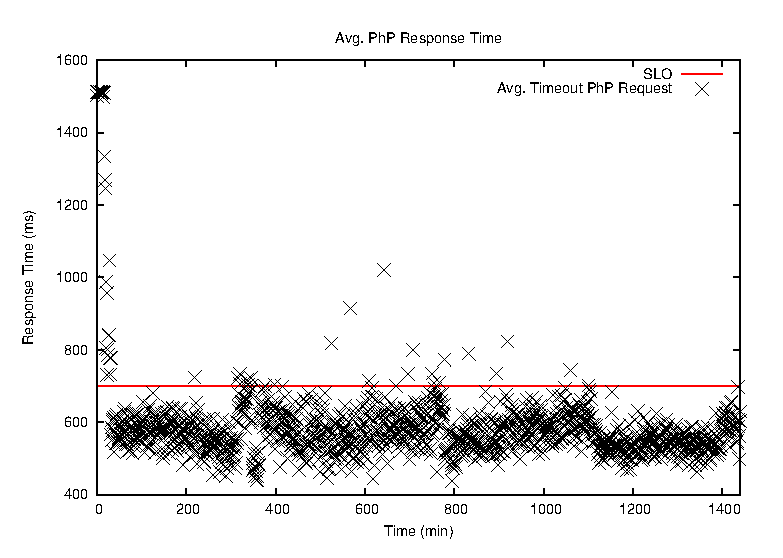
\includegraphics[width=0.49\textwidth, height=6cm]{./images/heterogeneous/avgTimeout_PhP_DLBweights}
\end{center}
\vspace{-5mm}
\caption{Response time on EC2-- Load-balancing Weights.}
\label{historyWeightEC2}
\end{figure}

\paragraph{Resource consumption.}
As explained above, the trigger-based algorithm sometimes initiates
series of scaling back quickly followed by scaling out operations, 
due to the fact that it does not use any history information that could
prevent these oscillations. This can be seen on Figure~\ref{resEC2},
in the time interval between \emph{t=400min} and \emph{t=500min}.
The feedback and dynamic load balancing algortithms have similar
and more stable patterns of resource consumption, which show the
benefits of using trend estimations and two-level threshold ranges.

%The resource usage on EC2 presents important changes, as shown on Figure~\ref{resEC2}. When using the trigger-based provisioning, the fluctuations in the system performance are explained as a result of a high frequency of scaling operations. In concrete, the fluctuations caused at the interval of time between \emph{t=400min} and \emph{t=500min} (see on Figure~\ref{naiveEC2}), match with the provisioning decisions made during the same interval of time on Figure~\ref{resEC2}. If we now pay attention to the feedback, and dynamic load-balancing weights algorithms, their resource consumptions are identical along the execution. Indeed, both algorithms decided to scale out the system during the interval of time comprised between \emph{t=1050min} and \emph{t=1400min}, to prevent future SLO violations that occurred when looking at the trigger-based algorithm on Figure~\ref{naiveEC2}. In particular, this situation demonstrates the benefits of using two-level threshold ranges to provide a predictive provisioning mechanism, thus improving the user experience.


\begin{figure}
\begin{center}
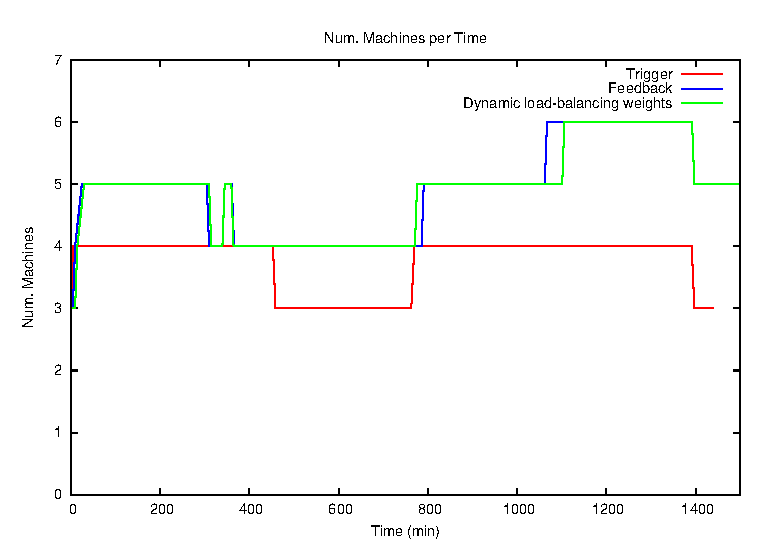
\includegraphics[width=0.49\textwidth, height=5cm]{./images/heterogeneous/numMachinesCompEC2}
\end{center}
\vspace{-5mm}
\caption{Resource consumption on EC2.}
\label{resEC2}
\end{figure}


\paragraph{Discussion.}
In order to have a better estimation of the algorithms' performance, we 
ran the experiments on Amazon EC2 a second time. The results of the two 
runs are summarized in Table~\ref{summaryEC2}, where we show the percentage
of SLO violations from the total number of requests, the number of
provisioning decisions (scaling out or back) taken by the algorithms
and an estimation of the cost of runnning the VMs in Amazon EC2.

Firstly, we noticed performance differences between the two runs of the
experiments, which are due to the fact that each experiment was run on
a different set of VMs from EC2. The trigger-based alogrithm in particular
is quite sensitive to small changes in the VM characteristics: since it
uses only one set of thresholds and no information about the workload
trend, it easily becomes unstable and may behave differently from one
run to another.

Secondly, both runs show significant differences between the trigger-based
algorithm on one hand, and the feedback and dynamic load balancing on
the other hand. The results show that using a few euristics as in the last
two algorithms can help in improving the performance and stability
of the system. We did not obtain however significant differences
between the feedback and the dynamic load balancing algorithm. The last
algorithm uses the additional technique of dynamically adjusting the
load balancing weights, but the the VMs participating in the experiments 
had relatively similar performance and adjusting their weights only
made a small difference. On other infrastructures that are more heterogeneous
than Amazon EC2, the dynamic load balancing technique may bring
a greater performance improvement.  

We also note that the cost of the trigger-based algorithm is slightly
lower than the cost of the other two algorithms. This algorithm
attempts more often to scale down the system, which explain the lower cost;
but on the other hand, this leads to more SLO violations and more
instability: many VM instances created and then shut down very soon. 

%The experiments on EC2 leads to several conclusions. The use of the trigger-based algorithm shows again how aggressive provisioning increases the resource consumption and the chances of degraded application performance due to frequents scaling actions. These actions are triggered as an effect associated to the traffic and heterogeneity of the requests, when handling bursty workload conditions. On the other hand, the feedback and dynamic load-balancing algorithms constitute two robust provisioning models that offer an efficient resource consumption and keep stable the application performance during the trace execution. 

%Furthermore, the use of a dynamic load-balancing algorithm provided a more efficient distribution of the request-mix across servers, that reduced the SLO violations in a 6.3\%. Hence, the main objective behind of this algorithm is to tackle the degradations caused by the workload heterogeneity.


%{\scriptsize
%\begin{table}
%\begin{center}
  %  \begin{tabular}{ | l | c | c |}
  %  \hline
  % \textbf{Algorithm}   & \textbf{DAS4} & \textbf{EC2}   \\ \hline
  %  Trigger-based & 3808 &  30357    \\ \hline
  %  Feedback &	2601 & 17856 \\ \hline
 %   Dynamic load-balancing   & -- & 15931\\ \hline
%\textbf{Num. of requests}  & 384501 & 438430  \\ \hline
  %  \hline
	
 %   \end{tabular}
%\end{center}
%\caption{SLO violations at the client's side (1500ms).}
%\end{table}
%}

\begin{table*}\label{summaryEC2}
  {\scriptsize 
\begin{center}
    \begin{tabular}{  | c | c | c | c | c | c | c | c | c |}
    \hline
    \multicolumn{3}{|c|}{ \textbf{Trigger}  } & \multicolumn{3}{|c|}{ \textbf{Feedback} }&  \multicolumn{3}{c|}{ \textbf{Load-balancing}  }   \\ \hline 
 \textbf{SLO Violations}& \textbf{Decisions} & \textbf{Cost} & \textbf{SLO Violations} & \textbf{Decisions} & \textbf{Cost} & \textbf{SLO Violations} & \textbf{Decisions} & \textbf{Cost} \\ \hline
  6.92\% & 14 & 7.5 &  4.07\%  & 8 & 7.7 &  3.63\% & 8 & 7.7  \\ \hline
  13.7 \% & 28 & 7.86 &  3.96\%  & 8 & 8.4 &  4.07\% & 8 & 8.32  \\ \hline
 \end{tabular}
\end{center}
\vspace{-5mm}
\caption{Analysis of results on EC2}
}
\end{table*}



%\subsection*{Discussion}

As a conclusion, we found from our experiments that a simple trigger-based
provisioning mechanism does not handle workload variation well and
in some situations causes instability, by changing the number of
provisioned VMs often in short time intervals. This behaviour has a 
negative effect on the application's response time, leading to violations
of the SLO.

By using a few techniques that are relatively easy to implement (like
estimating the workload's trend for the last 30 minutes and using
two levels of thresholds for the provisioning metrics) we showed that
we can significantly reduce the number of SLO violations and
obtain more stability. Although there is still room for improvement
in our techniques, from the experimental results we can draw the
conclusion that implementing provisioning mechanisms that go
beyond simple triggers is effective and should be considered
when hosting a cloud application.

%Generally, the result of our measurements show how the behavioral performance pattern and the resource consumption vary depending on the infrastructures on which we ran our experiments. Different hardware configurations such as those provided by DAS-4 and EC2, offer two distinct scenarios to validate our provisioning algorithms.  In these experiments, we demonstrate how trigger-based provisioning mechanisms can affect the system performance instead of improving it, as well as are wasteful in terms of resource usage. Furthermore, we show how a dynamic load-balancing technique, although intrusive, can be included and used without producing performance alterations. In fact, this technique slightly reduced the number of SLO violations in comparison with the results obtained using feedback algorithm. Finally, we also present the benefits by using feedback and dynamic load-balancing weights provisioning algorithms which aims to find the trade-off between the accuracy and cost savings. 

%However, there is room for improvement using the dynamic load-balancing weights algorithm, as some  workload alterations could not be handled during the trace execution.

%the flexible threshold ranges were pre-defined before execution for all VMs. These threshold values might be %changed depending the type of instance to be provisioned. Therefore, we believe that offline profiling techniques %may be used to define these values depending of the type of instance, thus improving the effectiveness of our %predictions.

%Today's resource provisioning systems define SLO's based on desirable threshold values for an application (CPU %$<$ 70\% and resp. time $<$= 700ms). However, these threshold values change depending the type of instance %to be provisioned (\emph{i.e.,} small instances 200 $<$ resp. time $<$ 500, while medium instances 200 $<$ %response time $<$ 600). In order to improve the accuracy of these algorithms, we consider that provisioning %decisions have to take into account two threshold ranges: (i) desirable threshold values for the whole application; %(ii) specific threshold values for each machine. Thus, to determine these machine-specific threshold values, offline %profiling techniques have to train during a period of time 








\section{Conclusion}
\label{sec:conclusion}
\label{sec:conclusion}



Nowadays cloud infrastructures offer a plethora of distinct hardware configurations for rent and price, we argued that autoscaling systems can use this diversity to better fulfill the SLA requirements without dramatically raising the operational cost. This has special importance for enterprises where a decrease in the user base led to a reduction in revenue, or for cloud providers where penalties paid due to SLO violations have a revenue impact. We proposed a novel autoscaling approach for cloud applications that provisions the most appropriate hardware configuration according to the customer requirements. This system benefits from cloud heterogeneity and online profiling techniques to find a scaling plan adapted to the QoS and current workload requirements. By considering factors such as SLO fulfillment or infrastructure cost, our system minimizes the performance degradations even under large and temporal workload variations. We implemented an autoscaling system that has been successfully deployed in multiple clouds. We evaluated our system in a realistic scenario showing the benefits by selecting a configuration that mitigates the performance degradations even under bursty workload. Nevertheless, these benefits could also be observed along the whole execution of a workload trace. In the future we plan to extend our system by supporting a bigger number of hardware configurations and by optimizing 
the dynamic load balancing mechanism. Similarly, we want to further study the financial impact of combining different hardware configurations.


% integrating a neural network forecasting model
% support for more types of instances.


%It is necessary to highlight the impotance of autoscaling systems that exploits the heterogeneity of the cloud infrastructures when provisioning applications.

%cheapest configuration doesn't have to be efficient. Tradittional system scale out and back using small instances.






\section*{Acknowledgments}

This work was partially funded by the FP7 Programme of the European
Commission in the context of the Contrail project under Grant
Agreement FP7-ICT-257438 and the Harness project under Grant Agreement
318521.


\bibliographystyle{IEEEtran}
\bibliography{main}


\end{document}
